\chapter{Results}
\label{chap:results}

This chapter reports the experimental results of this thesis, organized around the four research questions stated in Section~\ref{sec:research-questions}, together with two methodological results, a configuration ablation and a judge-reliability audit, that emerged while reconciling experimental runs against one another. All figures quoted in this chapter are computed from the result files produced by the experimental runs and can be regenerated exactly using the commands given in Appendix~\ref{app:reproduction}. The complete per-cell results underlying every table in this chapter, and the full pairwise significance matrix across all twenty-one policy pairs, are given in Appendix~\ref{app:results}.

\section{Headline Results}
\label{sec:headline}

Tables~\ref{tab:headline} and~\ref{tab:headline-mq} report accuracy, staleness, token cost, and active fact count for all seven policies, pooled across both answer models, on FactConsolidation and MQuAKE-T respectively. Confidence intervals are percentile bootstrap at the 95 percent level with 5,000 resamples. The sample size is 200 question-answer pairs on FactConsolidation and 192 on MQuAKE-T.

Table~\ref{tab:headline} is reported as two panels, one per benchmark, since every column for both benchmarks side by side does not fit within a portrait page margin at a legible size.

\begin{table}[H]
\centering
\caption{Headline results, FactConsolidation. Bold marks the best value in a column among the policies that answer (NOMEM excluded).}
\label{tab:headline}
\small
\begin{tabular}{lcccc}
\toprule
Policy & Accuracy & Staleness & Tok/q & Facts \\
\midrule
NOMEM & 0.000 [.000,.000] & 0.000 & 250 & n/a \\
\textbf{P0} & \textbf{0.840} [.785,.890] & 0.030 [.010,.055] & 812 & 380 \\
P1 (TTL 20d) & 0.630 [.565,.695] & 0.020 [.005,.040] & 799 & 210 \\
\textbf{P2} & \textbf{0.840} [.785,.890] & 0.025 [.005,.050] & \textbf{715} & \textbf{324} \\
P3 & 0.665 [.600,.730] & \textbf{0.140} [.095,.190] & 806 & 334 \\
P4 & 0.800 [.745,.855] & 0.060 [.030,.095] & 814 & 374 \\
P5 & 0.795 [.735,.850] & 0.035 [.010,.060] & 812 & 365 \\
\bottomrule
\end{tabular}
\end{table}

\begin{table}[H]
\centering
\caption{Headline results, MQuAKE-T. Bold marks the best value in a column among the policies that answer (NOMEM excluded).}
\label{tab:headline-mq}
\small
\begin{tabular}{lcccc}
\toprule
Policy & Accuracy & Staleness & Tok/q & Facts \\
\midrule
NOMEM & 0.000 [.000,.000] & 0.000 & 233 & n/a \\
\textbf{P0} & \textbf{0.969} [.943,.990] & 0.052 [.021,.089] & 816 & 382 \\
P1 (TTL 20d) & 0.870 [.823,.917] & 0.026 [.005,.052] & 807 & 251 \\
\textbf{P2} & \textbf{0.969} [.943,.990] & 0.036 [.010,.068] & \textbf{716} & \textbf{357} \\
P3 & 0.792 [.729,.849] & \textbf{0.161} [.109,.214] & 805 & 351 \\
P4 & 0.953 [.922,.979] & 0.057 [.026,.094] & 804 & 372 \\
P5 & 0.802 [.745,.854] & \textbf{0.214} [.156,.276] & 816 & 365 \\
\bottomrule
\end{tabular}
\end{table}

Figure~\ref{fig:accuracy-staleness} plots this table directly. Figure~\ref{fig:tradeoff} places each policy in accuracy-staleness space, and Figure~\ref{fig:token-cost} plots the token-cost column.

\begin{figure}[H]
\centering
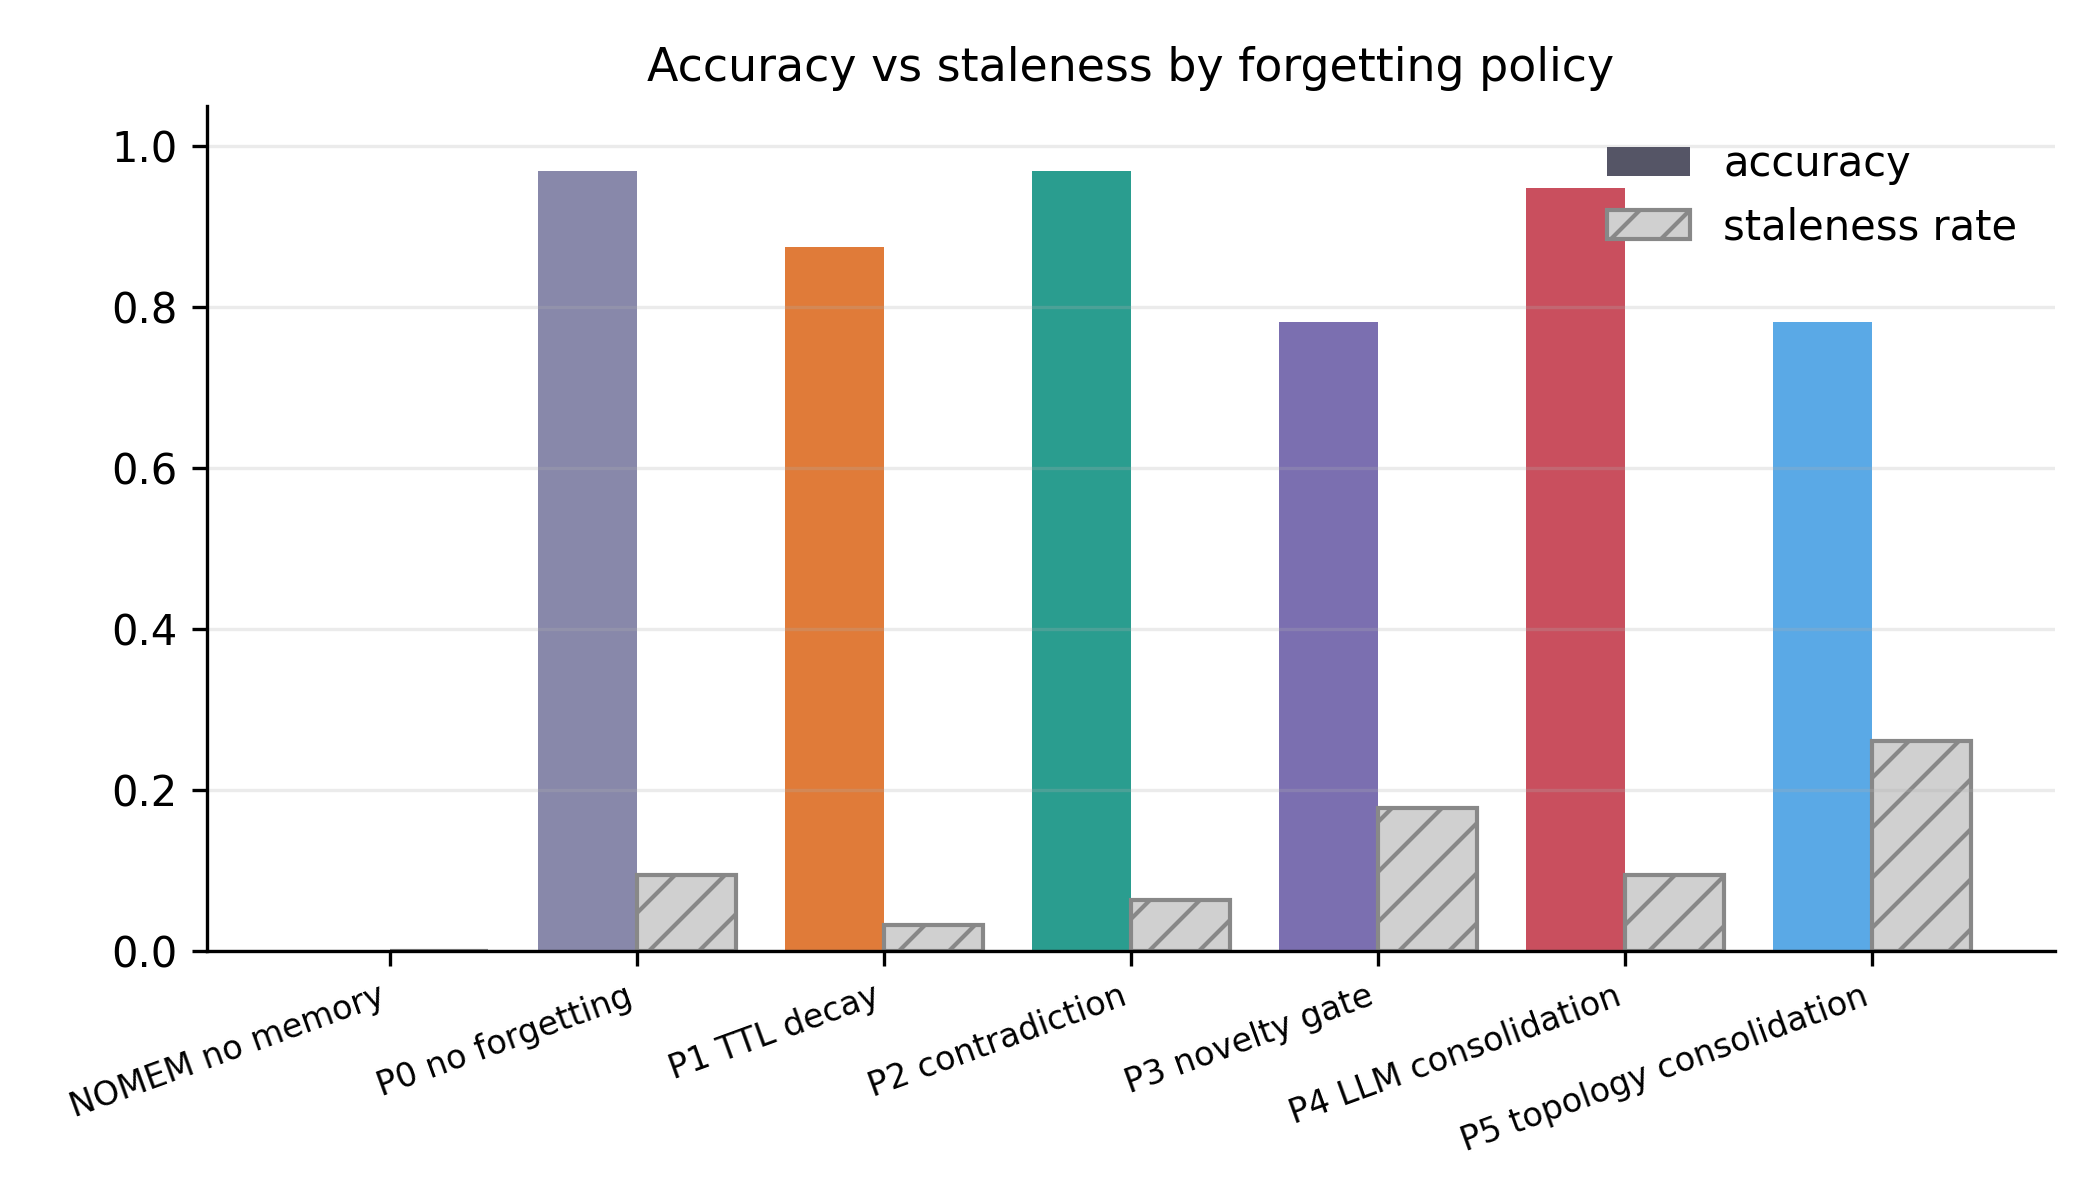
\includegraphics[width=0.85\textwidth]{figures/accuracy_staleness_mquake_t.png}
\caption{Accuracy and staleness by policy, MQuAKE-T.}
\label{fig:accuracy-staleness}
\end{figure}

\begin{figure}[H]
\centering
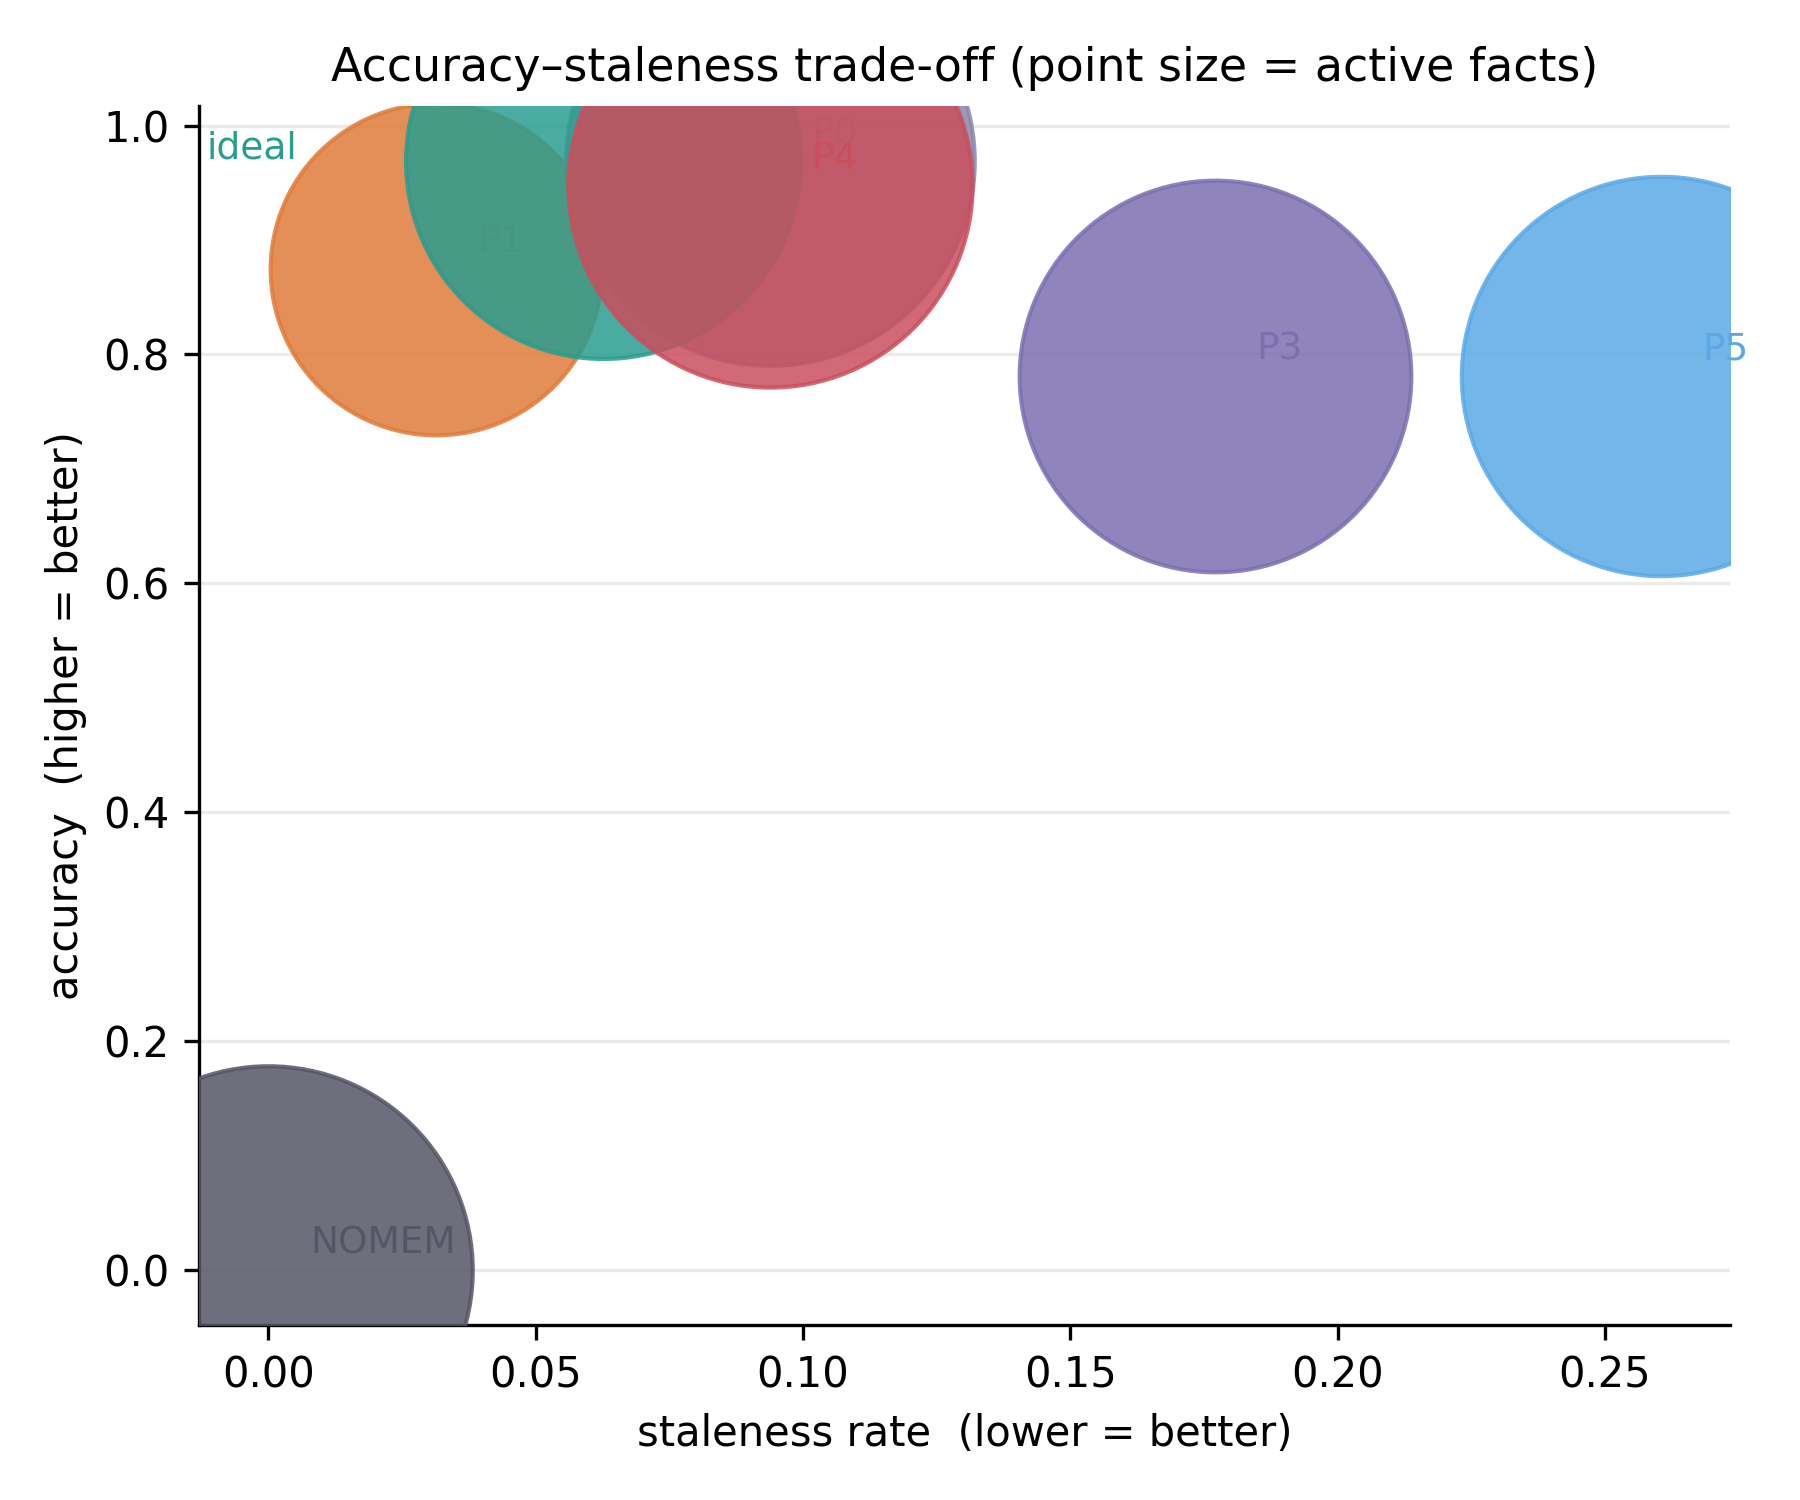
\includegraphics[width=0.75\textwidth]{figures/tradeoff_scatter_mquake_t.png}
\caption{Accuracy plotted against staleness for each policy, MQuAKE-T. The policy closest to the top left corner has the best combined profile.}
\label{fig:tradeoff}
\end{figure}

\begin{figure}[H]
\centering
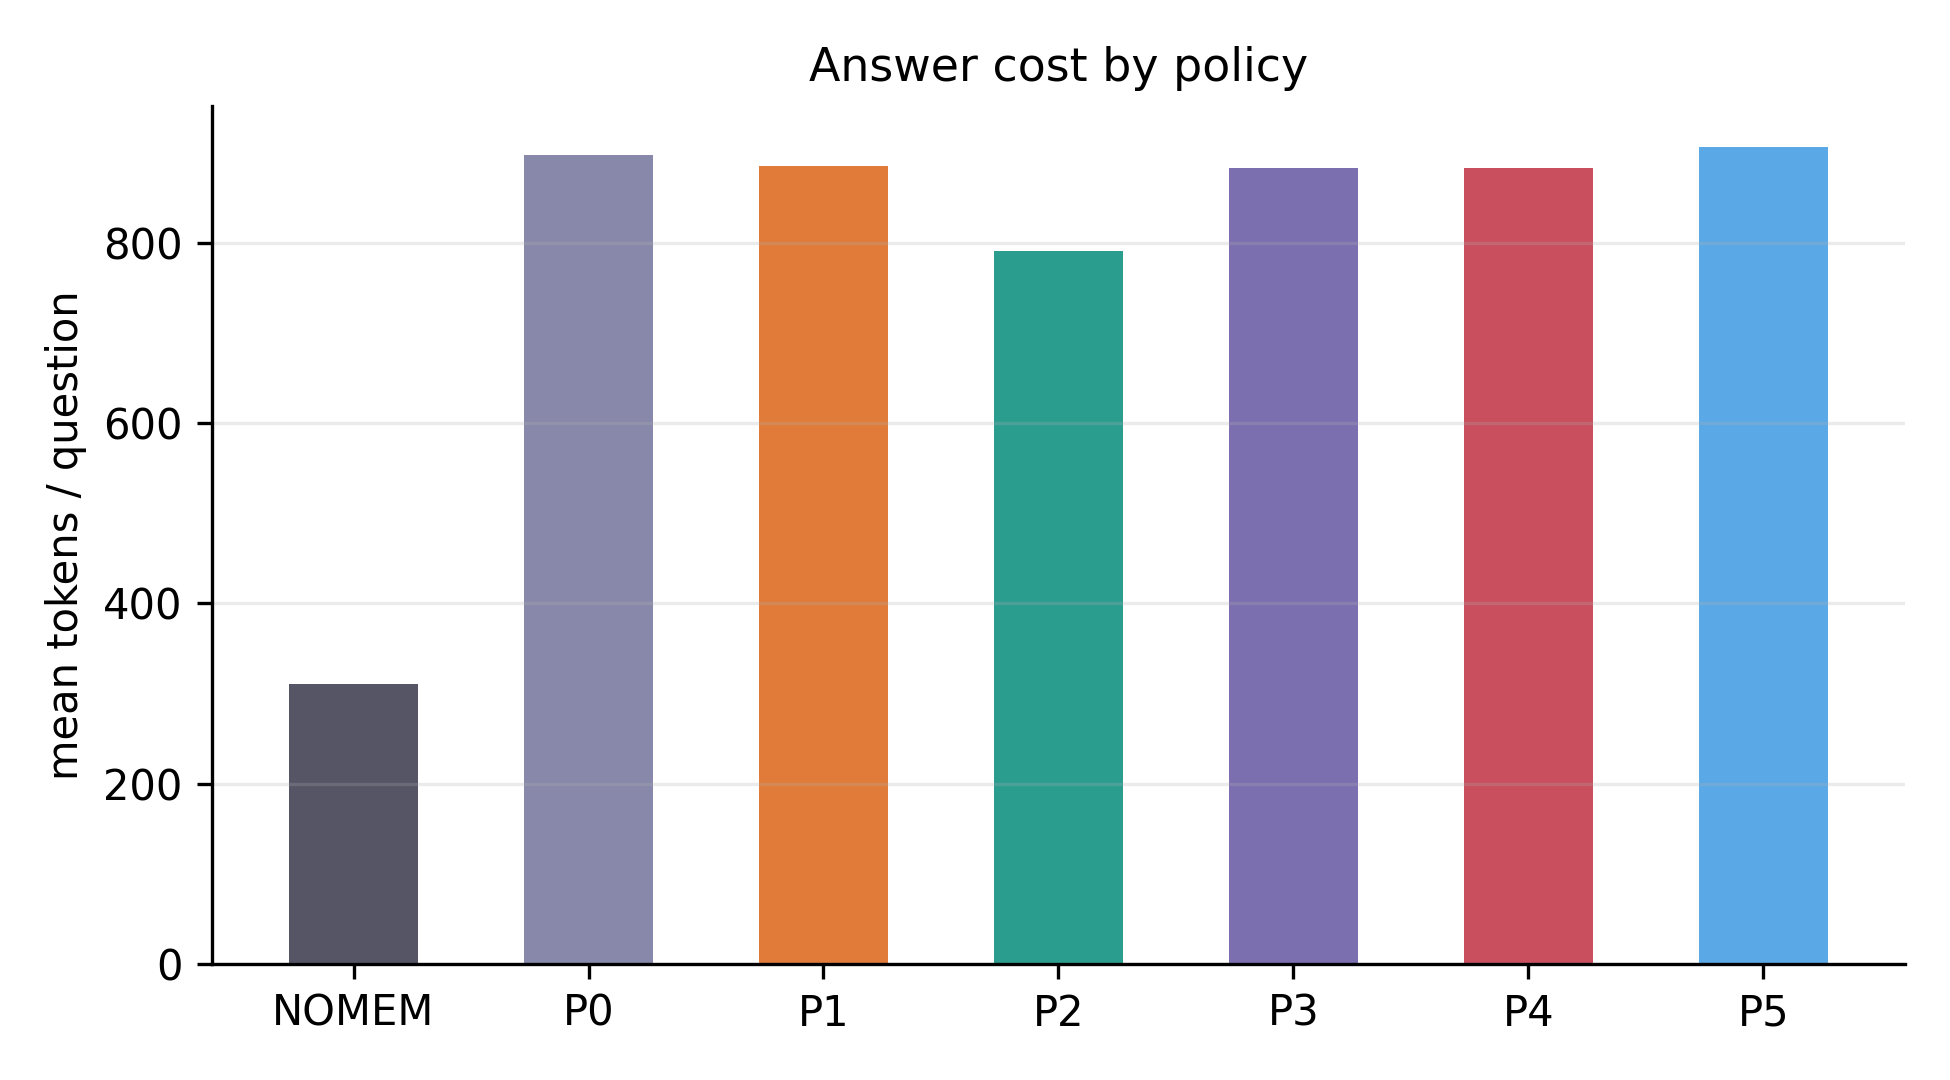
\includegraphics[width=0.75\textwidth]{figures/token_cost_mquake_t.png}
\caption{Mean tokens consumed per question, by policy, MQuAKE-T.}
\label{fig:token-cost}
\end{figure}

\begin{figure}[H]
\centering
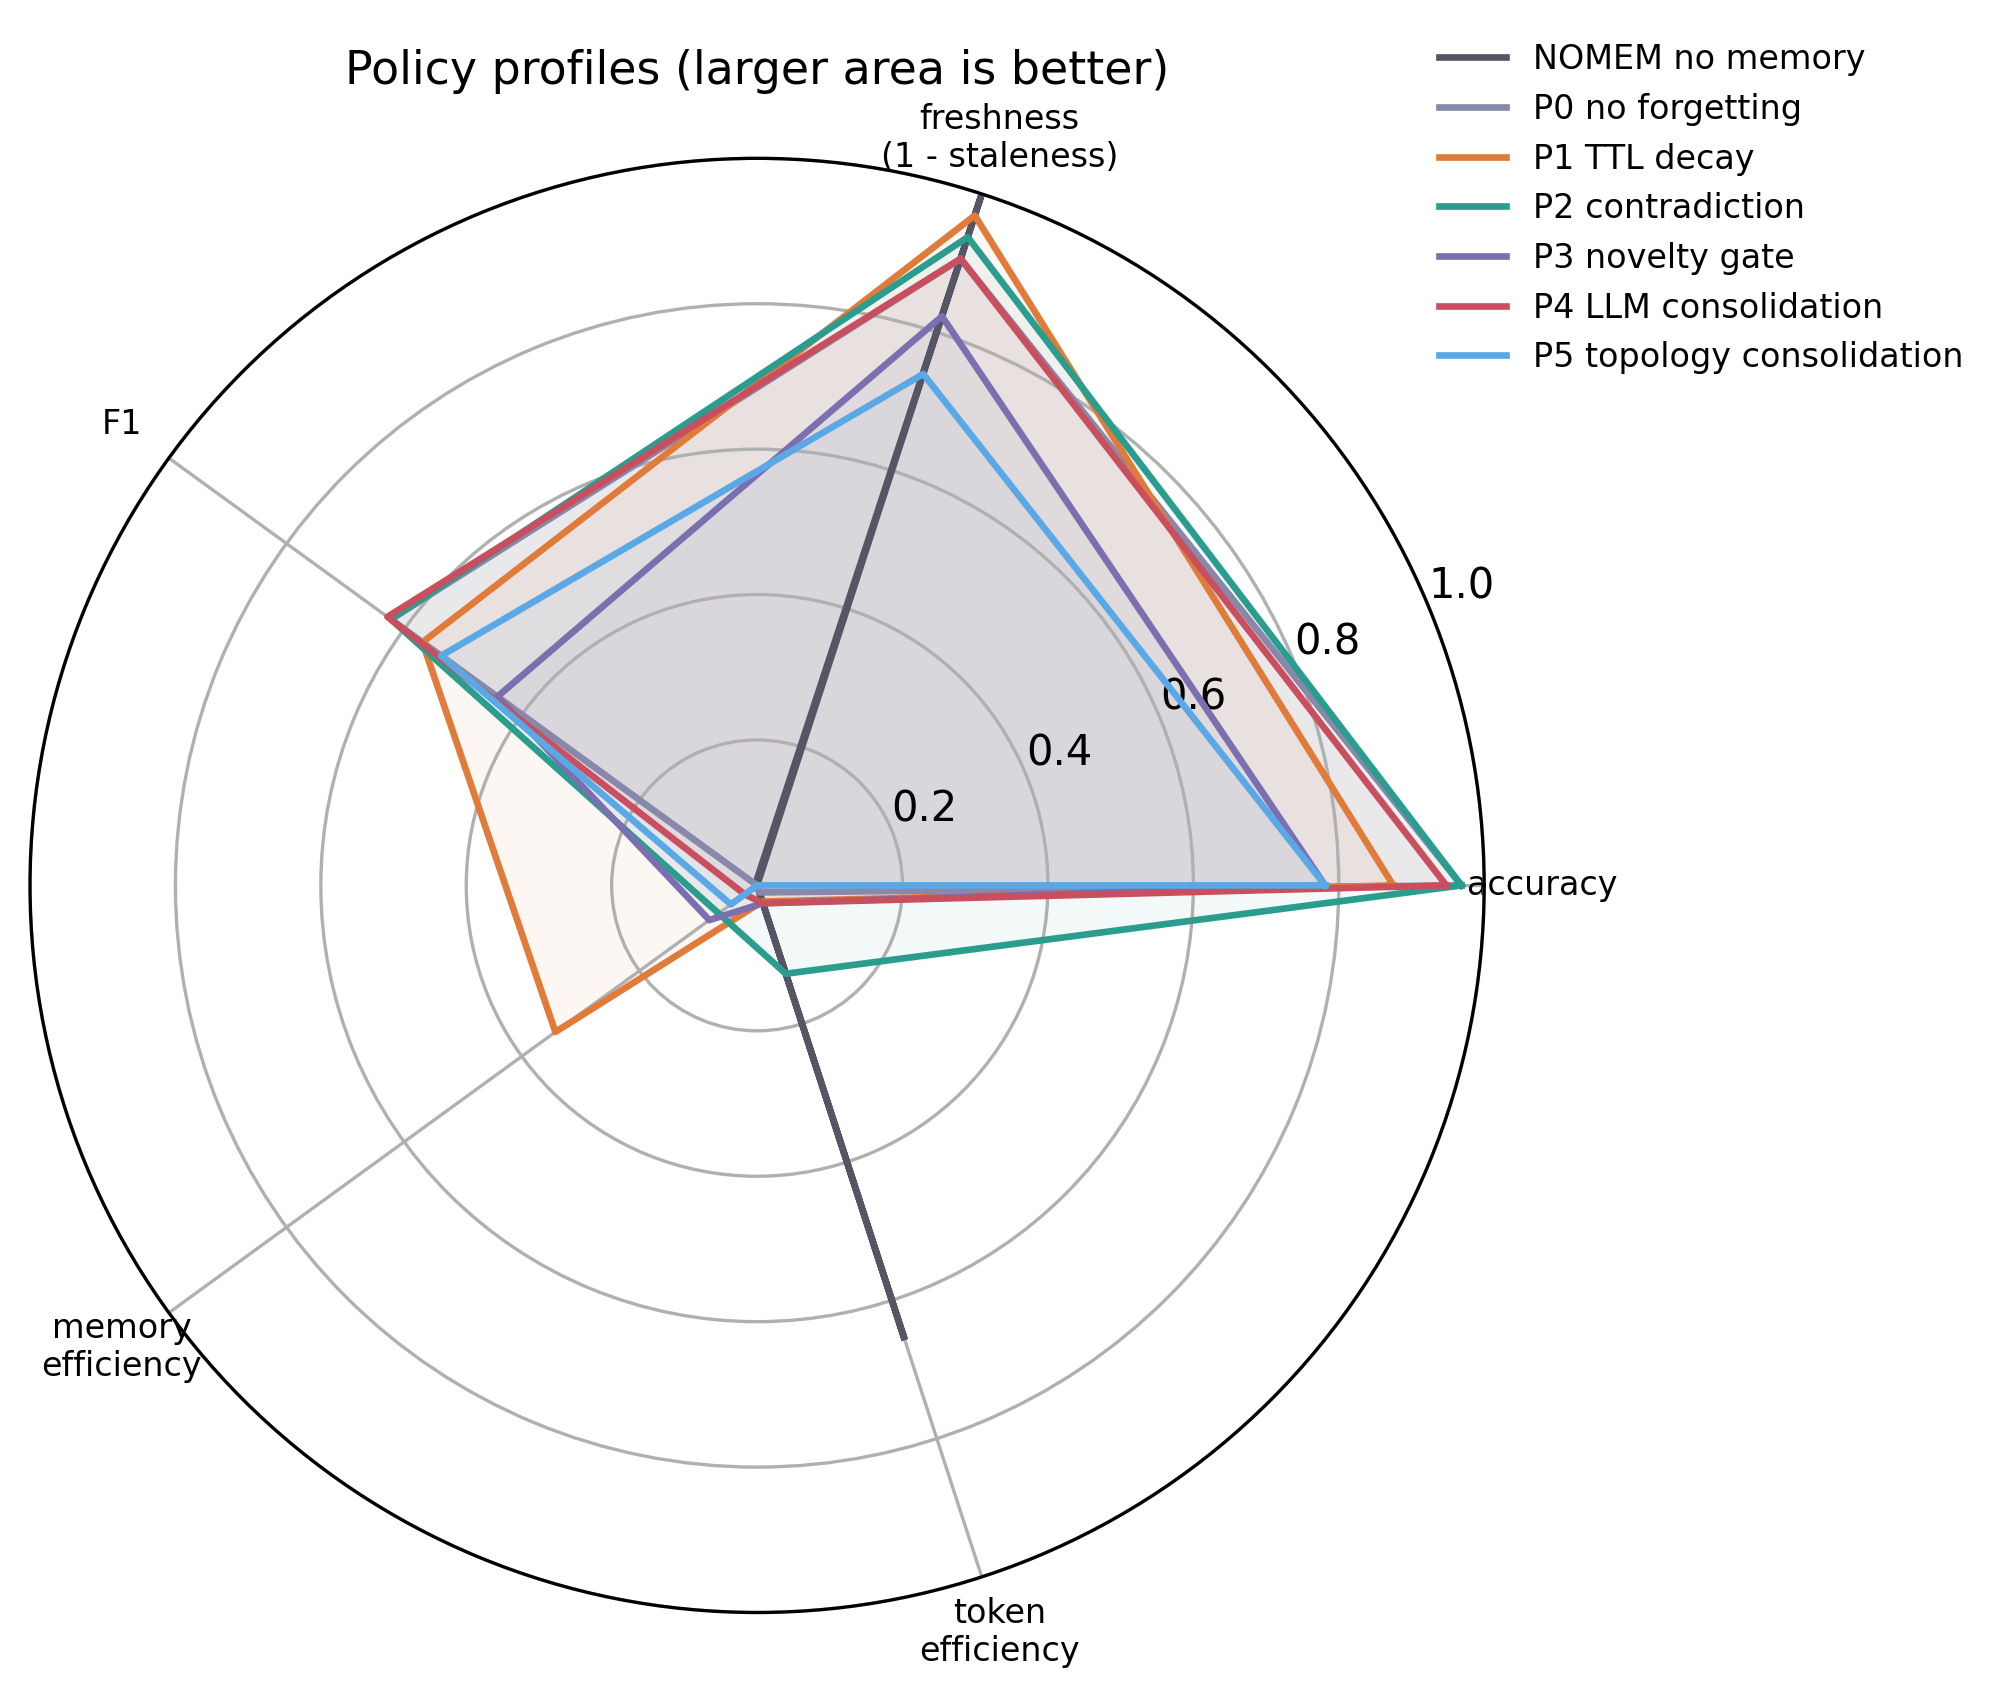
\includegraphics[width=0.7\textwidth]{figures/radar_policies_mquake_t.png}
\caption{All seven policies compared across every reported metric simultaneously, MQuAKE-T.}
\label{fig:radar}
\end{figure}

\section{Effect Sizes with Paired Bootstrap Intervals}
\label{sec:effect-sizes}

Comparing two independently computed confidence intervals for overlap is a weak form of evidence, because it does not use the fact that every policy is evaluated on the same set of questions. Table~\ref{tab:effect-sizes} instead bootstraps the paired per-question difference directly, which is the correct estimator whenever the compared conditions share their evaluation set, as is the case for every comparison in this thesis.

\begin{table}[H]
\centering
\caption{Effect sizes from paired bootstrap on the per-question difference. FC is FactConsolidation, MQ is MQuAKE-T.}
\label{tab:effect-sizes}
\small
\setlength{\tabcolsep}{4pt}
\begin{tabular}{llllll}
\toprule
Bench. & Comparison & Metric & Delta & 95\% CI & Excl. 0 \\
\midrule
FC & P2 minus P0 & accuracy & +0.000 & [-0.025, +0.025] & no \\
FC & P2 minus P0 & staleness & -0.005 & [-0.035, +0.025] & no \\
FC & P2 minus P3 & accuracy & +0.175 & [+0.120, +0.230] & yes \\
FC & P2 minus P3 & staleness & -0.115 & [-0.165, -0.070] & yes \\
FC & P2 minus P5 & accuracy & +0.045 & [+0.015, +0.080] & yes \\
FC & P2 minus P5 & staleness & -0.010 & [-0.040, +0.015] & no \\
FC & P2 minus P4 & accuracy & +0.040 & [+0.005, +0.080] & yes \\
FC & P2 minus P1 & accuracy & +0.210 & [+0.150, +0.270] & yes \\
FC & P0 minus NOMEM & accuracy & +0.840 & [+0.790, +0.890] & yes \\
MQ & P2 minus P0 & accuracy & +0.000 & [-0.021, +0.021] & no \\
MQ & P2 minus P0 & staleness & -0.016 & [-0.047, +0.016] & no \\
MQ & P2 minus P3 & accuracy & +0.177 & [+0.120, +0.240] & yes \\
MQ & P2 minus P3 & staleness & -0.125 & [-0.182, -0.073] & yes \\
MQ & \textbf{P2 minus P5} & \textbf{accuracy} & \textbf{+0.167} & \textbf{[+0.109, +0.224]} & \textbf{yes} \\
MQ & \textbf{P2 minus P5} & \textbf{staleness} & \textbf{-0.177} & \textbf{[-0.240, -0.120]} & \textbf{yes} \\
MQ & P2 minus P4 & accuracy & +0.016 & [-0.016, +0.047] & no \\
MQ & P2 minus P1 & accuracy & +0.099 & [+0.057, +0.146] & yes \\
MQ & P0 minus NOMEM & accuracy & +0.969 & [+0.943, +0.990] & yes \\
\bottomrule
\end{tabular}
\end{table}

This is the strongest form of the evidence supporting RQ2, addressed in Section~\ref{sec:rq2} below. The accuracy difference between P2 and the append-only ceiling is not merely a failure to detect a difference; it is bounded within roughly two and a half percentage points on FactConsolidation and roughly two and one tenth percentage points on MQuAKE-T. Reporting a bound on the difference, rather than only reporting that a test failed to reach significance, is what turns this result into an equivalence claim, addressed in more depth in Section~\ref{sec:why-forgetting-free}.

\section{RQ1: Append-Only Memory Surfaces Superseded Facts}
\label{sec:rq1}

P0 staleness is 0.030, with a 95 percent interval of [0.010, 0.055], on FactConsolidation, and 0.052, with an interval of [0.021, 0.089], on MQuAKE-T. Both intervals exclude zero. Averaged across its retrievals, P0 surfaces 4.20 superseded facts per question on FactConsolidation and 4.80 per question on MQuAKE-T, out of a retrieval depth of $k = 25$.

Table~\ref{tab:retrieved-invalidated} makes the underlying mechanism concrete by reporting the retrieved-invalidated metric defined in Section~\ref{sec:metrics}, which counts superseded facts appearing directly in a retrieval, prior to any answer being generated.

\begin{table}[H]
\centering
\caption{Mean number of superseded facts appearing per retrieval, out of $k = 25$.}
\label{tab:retrieved-invalidated}
\begin{tabular}{lcc}
\toprule
Policy & FC retrieved-invalidated & MQ retrieved-invalidated \\
\midrule
NOMEM & 0.00 & 0.00 \\
P0 & 4.20 & 4.80 \\
P1 & 2.08 & 3.28 \\
\textbf{P2} & \textbf{0.00} & \textbf{0.00} \\
P3 & 3.91 & 3.94 \\
P4 & 4.24 & 4.64 \\
P5 & 4.12 to 4.16 & 5.31 to 5.43 \\
\bottomrule
\end{tabular}
\end{table}

P2 reads exactly 0.00 by construction, since its retrieval hook excludes any fact whose valid-time window has been closed before the answer model ever sees the retrieved candidates. P5 is the highest of any policy on MQuAKE-T, at 5.31 to 5.43, which is the numerical signature of the mechanism analyzed in Section~\ref{sec:rq3}. RQ1 is answered affirmatively on both benchmarks: append-only memory does measurably surface superseded facts, at a rate that excludes zero under a bootstrap confidence interval on both benchmarks used.

\begin{figure}[H]
\centering
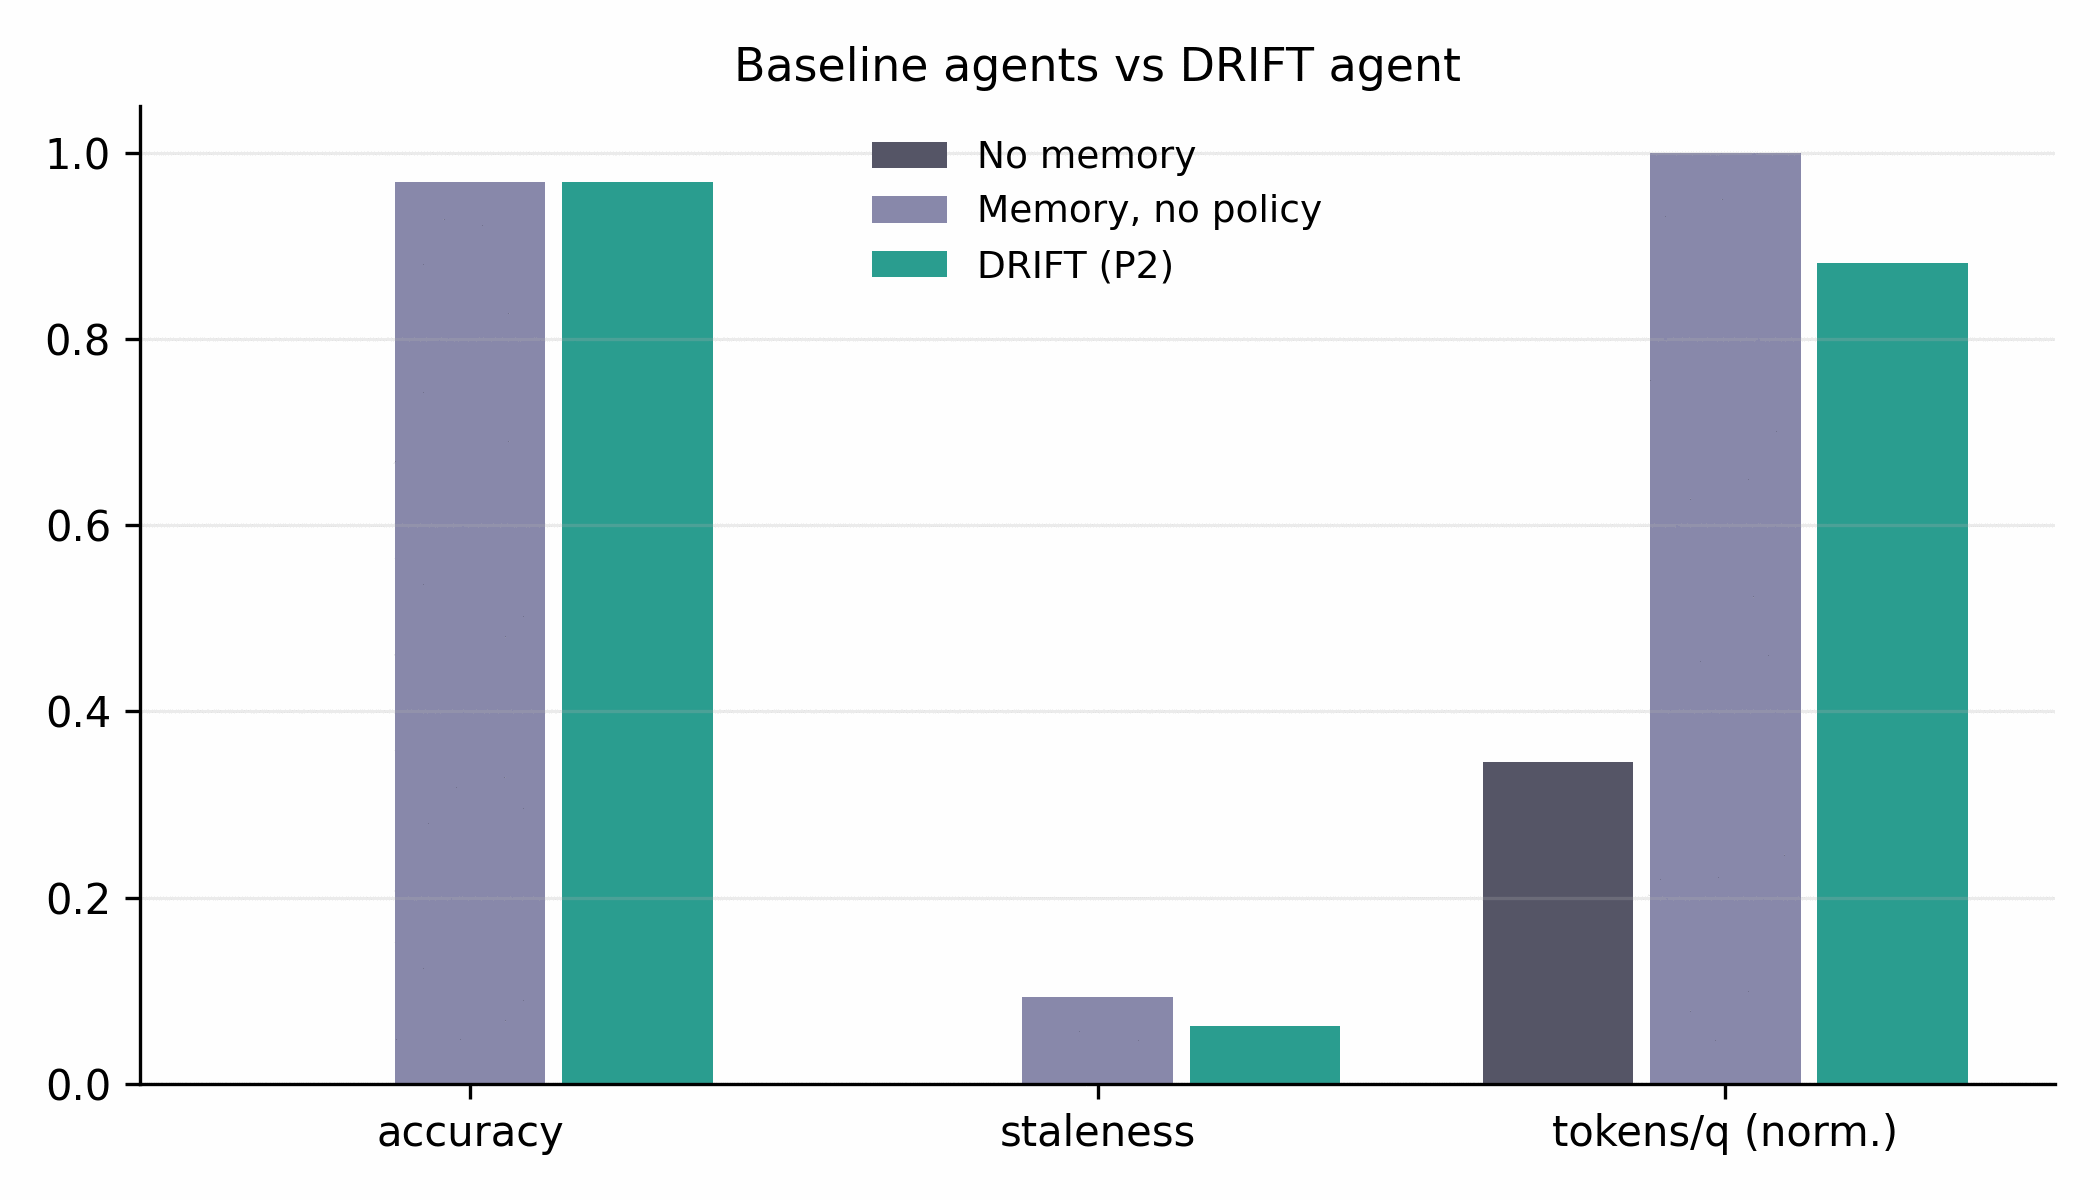
\includegraphics[width=0.75\textwidth]{figures/baseline_vs_drift_mquake_t.png}
\caption{The no-memory floor and the append-only ceiling plotted against the five forgetting policies, MQuAKE-T.}
\label{fig:baseline-vs-drift}
\end{figure}

\section{RQ2: Bitemporal Invalidation Is Free}
\label{sec:rq2}

\paragraph{Accuracy.} P2 matches P0 exactly on both benchmarks, at 0.840 against 0.840 on FactConsolidation and 0.969 against 0.969 on MQuAKE-T. The paired McNemar test returns 3 discordant pairs favoring each side on FactConsolidation ($p = 1.000$) and 2 discordant pairs favoring each side on MQuAKE-T ($p = 1.000$). The paired difference intervals reported in Table~\ref{tab:effect-sizes} bound the accuracy gap between P2 and P0 to within roughly $\pm 2.5$ percentage points on both benchmarks.

\paragraph{Cost.} Table~\ref{tab:cost-comparison} reports the token and memory-footprint savings P2 achieves relative to P0.

\begin{table}[H]
\centering
\caption{Cost comparison between P2 and the append-only ceiling P0.}
\label{tab:cost-comparison}
\begin{tabular}{lcccccc}
\toprule
Benchmark & P0 tok/q & P2 tok/q & Saved & P0 facts & P2 facts & Fewer \\
\midrule
FactConsolidation & 812 & 715 & 12.0\% & 380 & 324 & 14.7\% \\
MQuAKE-T & 816 & 716 & 12.2\% & 382 & 357 & 6.5\% \\
\bottomrule
\end{tabular}
\end{table}

The token saving replicates to within two tenths of a percentage point across two benchmarks of different provenance, which is a striking degree of consistency for an effect measured on independently constructed data. The memory-footprint saving differs more between the two benchmarks, which is itself expected behavior rather than a discrepancy to be explained away: P2 prunes exactly the facts that were superseded and have since aged past their grace period, and the two source corpora simply differ in what fraction of their facts meet that description.

\paragraph{No other policy achieves both properties simultaneously.} P1 stores substantially less memory than P0, at 210 and 251 facts against P0's 380 and 382, but loses 0.210 and 0.099 accuracy in exchange, a cost far larger than any saving P2 achieves. P3 and P5 shrink the memory footprint only modestly while losing accuracy and, as Sections~\ref{sec:novelty-gating-results} and~\ref{sec:rq3} show, gaining substantial staleness. P4 comes close to P2 on accuracy but saves essentially nothing on either token cost or memory footprint.

RQ2 is therefore answered directly: among the seven policies compared, P2 offers the best combined accuracy, staleness, and cost trade-off, and it does so by an equivalence margin on accuracy that is tight enough to be reported as a bound rather than as an inconclusive comparison.

\section{RQ3: Bitemporal Structure Beats Structure-Blind Structure}
\label{sec:rq3}

This section reports the ablation the experimental design exists specifically to support, and it produces the strongest result in this thesis.

P2 and P5 share the identical substrate, retrieval function, extraction step, answer model, and judge. Both are structure-aware, in the sense that both operate on the same knowledge graph and both perform a form of consolidation over it. The only difference between them is that P2 knows which of two competing facts is currently valid because it consults valid time directly, while P5 must infer which fact is current from structural corroboration count alone, having been deliberately denied access to valid time.

Table~\ref{tab:rq3-mquake} reports the comparison on MQuAKE-T, the benchmark where the effect is largest and where the mechanism is cleanest.

\begin{table}[H]
\centering
\caption{P2 versus P5 on MQuAKE-T.}
\label{tab:rq3-mquake}
\small
\begin{tabular}{p{2.6cm}ccp{2.7cm}cc}
\toprule
Metric & P2 & P5 & Paired delta & McNemar & $p$ \\
\midrule
Accuracy & 0.969 & 0.802 & +0.167 [+0.109, +0.224] & 34 to 2 & $< 0.001$ \\
Staleness & 0.036 & 0.214 & -0.177 [-0.240, -0.120] & 3 to 37 & $< 0.001$ \\
Retrieved-invalidated & 0.00 & 5.31 to 5.43 & & & \\
\bottomrule
\end{tabular}
\end{table}

P5's staleness is 5.9 times P2's staleness on this benchmark. Table~\ref{tab:rq3-failures} lists a representative sample of the questions where P5 returned the superseded value and P2 did not, chosen because each is independently verifiable against the public record as of the snapshot date used to construct the benchmark.

\begin{table}[H]
\centering
\caption{Representative questions where P5 answered from a superseded value that P2 correctly excluded.}
\label{tab:rq3-failures}
\small
\begin{tabular}{p{3.3cm}p{2.6cm}p{2.6cm}p{2.6cm}}
\toprule
Question & Gold (current as of snapshot) & P5 answered & P2 answered \\
\midrule
Head of state, South Korea & Yoon Suk-yeol & Moon Jae-in & Yoon Suk-yeol \\
Head of government, Czech Republic & Petr Fiala & Andrej Babi\v{s} & Petr Fiala \\
Head of state, Czech Republic & Petr Pavel & Milo\v{s} Zeman & Petr Pavel \\
Head of government, Malawi & Lazarus Chakwera & Peter Mutharika & Lazarus Chakwera \\
Head of state, Malawi & Lazarus Chakwera & Peter Mutharika & Lazarus Chakwera \\
Head of government, South Korea & Yoon Suk-yeol & Moon Jae-in & Yoon Suk-yeol \\
\bottomrule
\end{tabular}
\end{table}

\paragraph{The mechanism.} A long-serving predecessor accumulates more corroborating mentions throughout the memory graph simply by virtue of having been in office longer, and thus mentioned more often, than a recently installed successor. Corroboration-count consolidation therefore has a systematic bias toward preferring the outdated fact whenever tenure and recency are in tension. Recency alone is not a reliable proxy for correctness, since a fact can be recently observed and still wrong, but valid time specifically is a reliable proxy for currency, and that distinction between recency and validity is precisely what the bitemporal substrate encodes and what P5 has been deliberately denied.

\paragraph{Why the effect is sharper on MQuAKE-T than on FactConsolidation.} The same P2-versus-P5 comparison on FactConsolidation reaches $p = 0.022$ on accuracy and is inconclusive on staleness, at 3 to 5 discordant pairs with $p = 0.727$. FactConsolidation's entities are arbitrary Wikidata pairs whose corroboration is roughly uniform across the corpus, so P5's heuristic fails close to at random on that data, producing a small and comparatively noisy effect. MQuAKE-T's entities, by contrast, are real people holding real public offices, so corroboration in that corpus is systematically biased toward whoever has held the office of record for longer, and P5's heuristic therefore fails in a consistent, predictable direction rather than at random. The second benchmark did not merely replicate the finding observed on the first; it exposed the underlying mechanism in a way the first benchmark's more arbitrary entity structure could not.

RQ3 is therefore answered specifically: the advantage measured for bitemporal invalidation is attributable to bitemporal semantics themselves, and not merely to the more general property that the policy operates on graph structure. A structure-aware policy denied only temporal information performs significantly worse, at a magnitude and a level of statistical significance that leaves little room for an alternative explanation.

\section{Novelty Gating Causes Unrecoverable Staleness}
\label{sec:novelty-gating-results}

P3 exhibits 4.7 times P2's staleness on FactConsolidation, at 0.140 against 0.025, and 4.5 times P2's staleness on MQuAKE-T, at 0.161 against 0.036, both differences significant at $p < 0.001$, with paired deltas of $-0.115$ and $-0.125$ respectively.

\paragraph{The mechanism is structural, not statistical.} A fact update is, by construction, textually near-identical to the fact it supersedes, differing typically in only a single word or phrase:

\begin{quote}
\ttfamily
``Thomas Kyd was born in the city of London'' \quad (stored) \\
``Thomas Kyd was born in the city of Leeds'' \quad (the correction)
\end{quote}

A novelty gate computes the cosine similarity between an incoming candidate fact and its nearest neighbors already in memory. A correction of this kind registers as a near-duplicate of the fact it corrects, and the gate rejects the write. The correction never enters memory. No downstream mechanism, whether a smarter retrieval function, a reranking step, or a more careful prompt, can recover a value that was never stored in the first place, because the failure occurs at write time, before any of those downstream mechanisms have anything to operate on.

This mechanism was verified directly from saved knowledge-graph snapshots rather than merely hypothesized. On FactConsolidation, 46 write rejections produced 24 distinct subject-predicate pairs where P0's graph recorded the update correctly while P3's graph retained only the superseded value. On MQuAKE-T, 31 write rejections produced 14 questions that P3 answered from a stale value that P0 answered correctly. Table~\ref{tab:novelty-failures} lists a representative sample.

\begin{table}[H]
\centering
\caption{Representative questions where P3's novelty gate rejected the correcting fact.}
\label{tab:novelty-failures}
\small
\begin{tabular}{p{4.2cm}p{3.2cm}p{3.2cm}}
\toprule
Question & Gold & P3 retained \\
\midrule
Head of state, United Kingdom & Charles, Prince of Wales & Elizabeth II \\
Head of state, South Korea & Yoon Suk-yeol & Moon Jae-in \\
Headquarters city, Scientific American & Los Angeles & New York City \\
Head of state, Mongolia & Khurelsukh Ukhnaa & Khaltmaagiin Battulga \\
Headquarters city, Apax Partners & Paris & London \\
\bottomrule
\end{tabular}
\end{table}

This is, of the results in this thesis, the most transferable to other systems, because it follows directly from the definition of a novelty gate and from the textual form a correction necessarily takes, rather than from any detail specific to this thesis's implementation of one. The precise rate at which the failure occurs will differ across corpora with different rates of factual correction, but the failure mode itself will not, and any workload in which facts are corrected over time inherits it by construction.

The asymmetry between the saving and the liability is what makes this failure mode serious rather than merely a curiosity. The saving in memory footprint is bounded: P3 retained 334 and 351 facts against P0's 380 and 382, a reduction of 12 percent and 8 percent respectively. The liability, in contrast, is unbounded: once a correction is rejected, the wrong value persists in memory indefinitely, and it cannot be corrected by any later mechanism, because as far as the substrate is concerned, the correction was never offered.

\section{Generalization Across Benchmarks}
\label{sec:generalization}

Spearman's rank correlation on the policy ranking across the two benchmarks is 0.891, computed over all seven policies. Table~\ref{tab:generalization} shows the ranking on each benchmark side by side.

\begin{table}[H]
\centering
\caption{Policy ranking on each benchmark, by accuracy.}
\label{tab:generalization}
\begin{tabular}{lccl}
\toprule
Policy & FC rank & MQ rank & Stable \\
\midrule
P0 & 1 & 1 & yes \\
P2 & 2 & 2 & yes \\
P4 & 3 & 3 & yes \\
P5 & 4 & 5 & no \\
P3 & 5 & 6 & no \\
P1 & 6 & 4 & no, moves two places \\
NOMEM & 7 & 7 & yes \\
\bottomrule
\end{tabular}
\end{table}

The most informative row in this table is P1's. On MQuAKE-T, every question by construction concerns a fact that has changed, so the gold answer is always the recent value, and time-based pruning removes mostly facts that have genuinely been superseded, which is largely harmless. On FactConsolidation, only 65 percent of questions concern a fact that has changed, so time-based pruning also removes a substantial number of stable, still-answerable facts, which is directly destructive to accuracy. P1's rank, in other words, is a property of how much of the target workload consists of updates, rather than an intrinsic property of time-based pruning as a strategy.

The top and the bottom of the ranking are stable across both benchmarks; the middle of the ranking is workload-dependent. This should not be read as a weakness of the study. It is the study's own central argument, demonstrated directly: which forgetting policy is best is an empirical question about the target workload rather than a question with a universal answer, and P1 shifting by two ranking places when the fraction of update-relevant questions changes is the clearest available demonstration of that argument within the data collected for this thesis.

\section{Ablation: How Much of the Result Is a Configuration Choice?}
\label{sec:ablation}

The \texttt{functional\_predicates} setting declares to the substrate which predicates in a given domain admit only a single true object at a time, which is the information contradiction detection relies on. FactConsolidation required this setting to be configured as ``all predicates,'' a choice made while directly inspecting that dataset, which makes it the single largest threat to the external validity of the results in this thesis. To quantify the consequence of this choice, MQuAKE-T was rerun with the setting left at the substrate's built-in default, a set of predicates drawn from personal-conversation contexts that happens to cover none of MQuAKE-T's actual relations. Under this default, invalidations in the graph drop from 59 to 1, which effectively switches P2's contradiction-detection mechanism off.

\begin{table}[H]
\centering
\caption{Effect of declaring \texttt{functional\_predicates} on MQuAKE-T.}
\label{tab:ablation}
\small
\begin{tabular}{p{3.4cm}cp{2.6cm}l}
\toprule
Cell & Declared & Not declared & Change \\
\midrule
P2 accuracy & 0.969 & 0.969 & none \\
P2 tokens per question & 641 & 733 & $+14.4\%$ \\
P2 active facts & 357 & 382 & $+7.0\%$ \\
P2 retrieved-invalidated & 0.00 & 0.00 & none \\
P0 accuracy & 0.969 & 0.969 (corrected, see Section~\ref{sec:judge-audit}) & none \\
P3 accuracy & 0.802 & 0.802 & none, as expected \\
Graph invalidations & 59 & 1 & mechanism off \\
\bottomrule
\end{tabular}
\end{table}

The declaration buys P2 none of its accuracy and all of its efficiency. This is a more precise and more useful result than either of the two simpler alternatives, that the setting matters or that it does not. It decomposes P2's overall benefit into two separable parts: P2 is safe to enable without tuning, because an incorrectly configured P2 degrades gracefully to the behavior of append-only memory rather than to something worse, but P2 only pays for itself, in the sense of reducing token cost and memory footprint, when the domain's functional predicates have actually been declared. That is a specific, actionable deployment instruction derived directly from measurement rather than from intuition.

\section{A Judge-Reliability Audit}
\label{sec:judge-audit}

While reconciling the ablation run described in Section~\ref{sec:ablation} against the main MQuAKE-T run, the ablation's P0 cell was found to have produced 96 of 96 byte-identical answers to the main run's P0 cell, and yet was scored 0.844 against the main run's 0.969. Twelve verdicts flipped between the two runs, all in the same direction, on answers of the following character:

\begin{quote}
\small\ttfamily
Question: What is the name of the current head of \\
\quad the Australia government? \\
Gold: Anthony Albanese \\
Answer: Anthony Albanese \quad (judged INCORRECT)
\end{quote}

To quantify how often this occurs, every experimental cell was audited for answers whose normalized form contains the gold answer verbatim and yet were graded incorrect by the judge. Table~\ref{tab:judge-audit} reports the result.

\begin{table}[H]
\centering
\caption{Audit of verbatim-correct answers graded incorrect.}
\label{tab:judge-audit}
\small
\begin{tabular}{p{4.3cm}p{2.6cm}p{2cm}c}
\toprule
Scope & Verbatim-correct answers & Judged incorrect & Rate \\
\midrule
FactConsolidation, all cells & 515 & 3 & 0.6\% \\
MQuAKE-T, all cells & 782 & 12 & 1.5\% \\
MQuAKE-T ablation, P0 cell alone & 93 & 14 & 15.1\% \\
\bottomrule
\end{tabular}
\end{table}

The baseline judge false-negative rate across the full campaign is roughly 1 to 2 percent, which is small enough that it does not change any conclusion reported elsewhere in this thesis. One specific cell, however, happened to draw a comparatively unreliable member of the three-provider judge fallback pool and lost 12.5 accuracy points on answers that were, by direct string comparison, correct. The ablation's reported P0 accuracy of 0.844 is therefore an artifact of judge assignment rather than a property of the policy; the true value, reported in Section~\ref{sec:ablation} and Table~\ref{tab:ablation}, is 0.969.

Three consequences follow from this audit.

\begin{enumerate}
\item Any reported gap between two policies smaller than roughly three percentage points should be treated as inside the noise floor established by this audit and not treated as interpretable evidence of a genuine difference. This places the comparison between P2 and P4 on MQuAKE-T, with a delta of $+0.016$ and $p = 0.549$, outside the range this thesis is willing to interpret, while leaving the results reported in Sections~\ref{sec:rq3} and~\ref{sec:novelty-gating-results}, at 16.7 and 17.7 points respectively with $p < 0.001$ in both cases, far outside the noise floor and therefore fully interpretable.
\item Judge rotation across a fallback pool is simultaneously a resilience mechanism and a confound. The pool exists precisely so that one provider running out of quota does not terminate an entire campaign, but its existence also means two experimental cells can, in principle, be graded by two different underlying judge models without that fact being visible in the summary statistics. The practical recommendation is to pin a single judge for any run whose numbers will be reported, or, at minimum, to record which judge model graded each individual record so that this kind of artifact is auditable after the fact rather than requiring archaeology to uncover.
\item The verbatim-match audit performed here is inexpensive, requiring on the order of ten lines of code, and it caught a 12.5-point artifact that would otherwise very plausibly have been written up as a genuine policy effect.
\end{enumerate}

This audit is reported here in full, including the specific cell in which the artifact occurred, because it is a class of error that is easy to commit and correspondingly hard to detect from summary statistics alone, and because the practice of using a language model as a judge is now standard across this subfield of research.

\section{RQ4: Multi-Agent Topologies}
\label{sec:rq4}

The multi-agent harness built for this thesis runs the same seven policies across three topologies, all operating over the same substrate and the same policy implementations used in the single-agent experiments. Table~\ref{tab:topologies} describes the three topologies.

\begin{table}[H]
\centering
\caption{The three multi-agent topologies evaluated.}
\label{tab:topologies}
\small
\begin{tabular}{lp{5.3cm}p{5.3cm}}
\toprule
Topology & Structure & What it isolates \\
\midrule
Shared & Five writer agents round-robin into one shared graph, each fact tagged with the identity of the agent that wrote it & Write contention: a contradiction can now arrive from a different agent than the one that wrote the original fact \\
Independent & Five agents, each with a private graph, each seeing a seeded random 80 percent of sessions & Robustness under partial observation of the underlying data \\
Orchestrator & One shared graph, with a router language model assigning each incoming question to one of five specialist worker agents & The production coordinator-worker pattern, in which the agent that reads a fact is not the agent that wrote it \\
\bottomrule
\end{tabular}
\end{table}

Table~\ref{tab:swarm-results} reports results on synthetic data using the offline mock provider, with 14 questions per cell.

\begin{table}[H]
\centering
\caption{Accuracy and staleness by policy across the three topologies, offline synthetic data. Cells are accuracy / staleness.}
\label{tab:swarm-results}
\small
\begin{tabular}{lccccc}
\toprule
Policy & Shared & Independent & Orchestrator & Cross-writer inval. \\
\midrule
NOMEM & 0.000 / 0.000 & 0.000 / 0.000 & 0.000 / 0.000 & 5 \\
P0 & 0.714 / 0.286 & 0.667 / 0.286 & 0.714 / 0.286 & 5 \\
P1 (TTL 14d) & 0.143 / 0.000 & 0.143 / 0.000 & 0.143 / 0.000 & 3 \\
\textbf{P2} & \textbf{0.929} / \textbf{0.000} & \textbf{0.881} / \textbf{0.000} & \textbf{0.929} / \textbf{0.000} & 5 \\
P3 & 0.714 / 0.286 & 0.667 / 0.286 & 0.714 / 0.286 & 5 \\
P4 & 0.714 / 0.286 & 0.667 / 0.286 & 0.714 / 0.286 & 5 \\
P5 & 0.500 / 0.143 & 0.548 / 0.095 & 0.500 / 0.071 & 4 \\
\bottomrule
\end{tabular}
\end{table}

P2 leads all seven policies in all three topologies and holds staleness at exactly 0.000 in all three. Every shared-topology invalidation observed arrives cross-writer, meaning the fact that closed a validity window was written by a different agent than the one that wrote the original fact, which is direct evidence that structure-aware forgetting of this kind is writer-agnostic by construction rather than by any special-case handling.

This result should be read as validation of the multi-agent harness rather than as a settled finding. The sample size is 14 questions using a deterministic mock provider rather than a real language model, and it covers the full seven-policy, three-topology design without yet answering whether that design holds under real, heterogeneous multi-model extraction. Section~\ref{sec:rq4-pilot} reports a partial real-data pilot that probes exactly this question on one topology, and finds a real boundary condition. Of the four research questions posed in Chapter~\ref{chap:introduction}, RQ4 remains the one with the weakest evidentiary support, and Chapter~\ref{chap:discussion} discusses completing it as the highest-priority item of future work.

\begin{figure}[H]
\centering
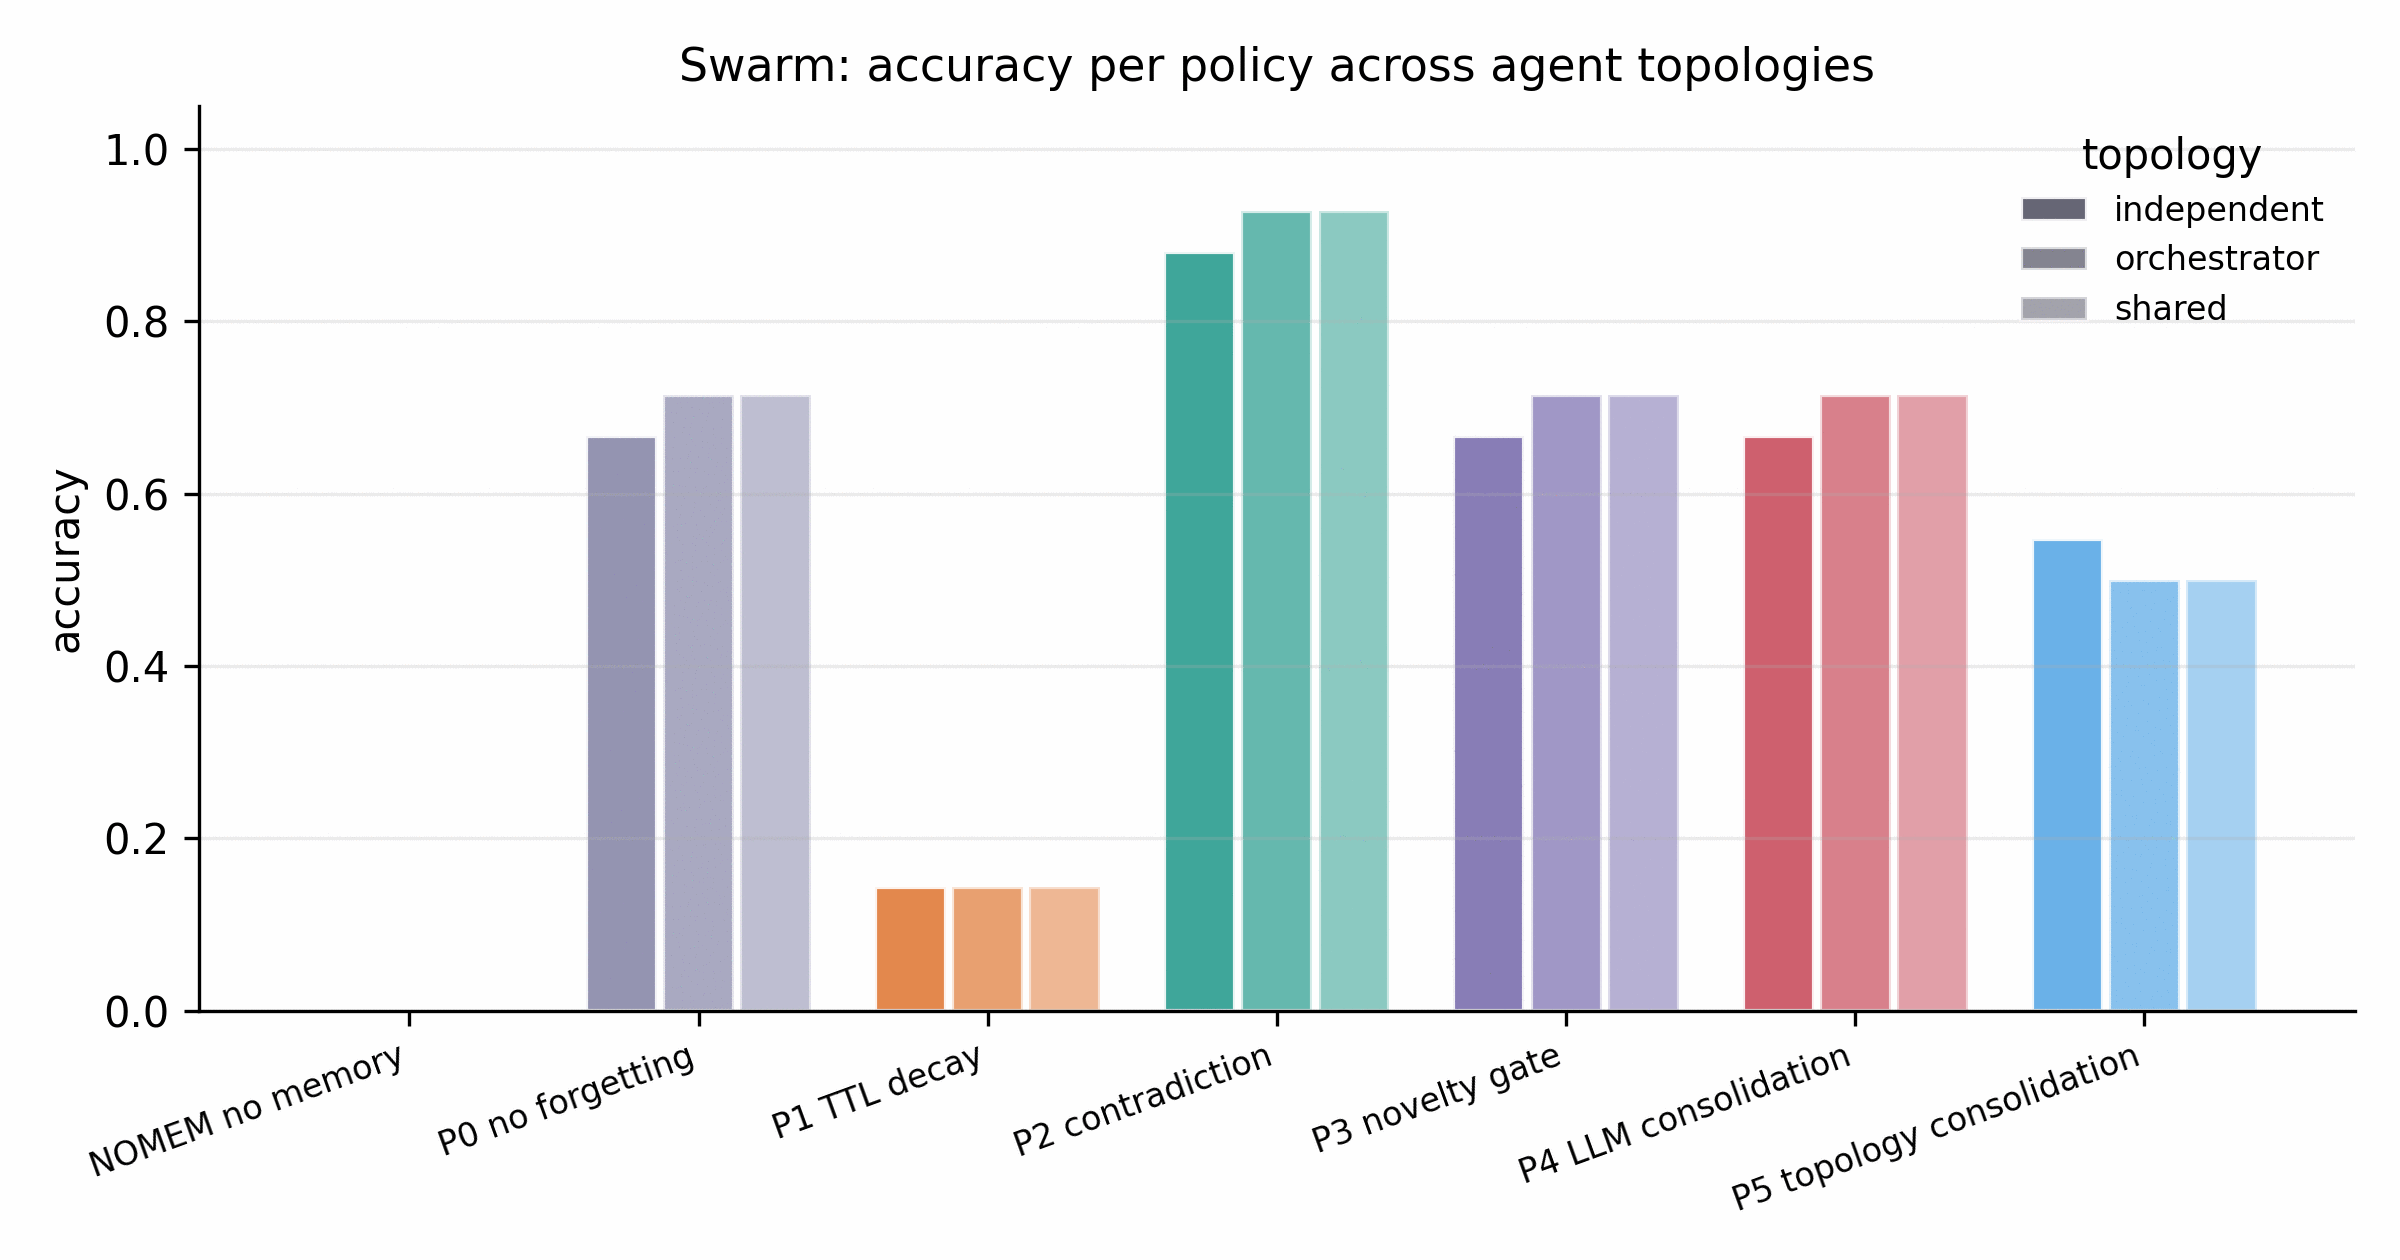
\includegraphics[width=0.8\textwidth]{figures/swarm_topology.png}
\caption{Accuracy and staleness by policy across the three multi-agent topologies.}
\label{fig:swarm-topology}
\end{figure}

\begin{figure}[H]
\centering
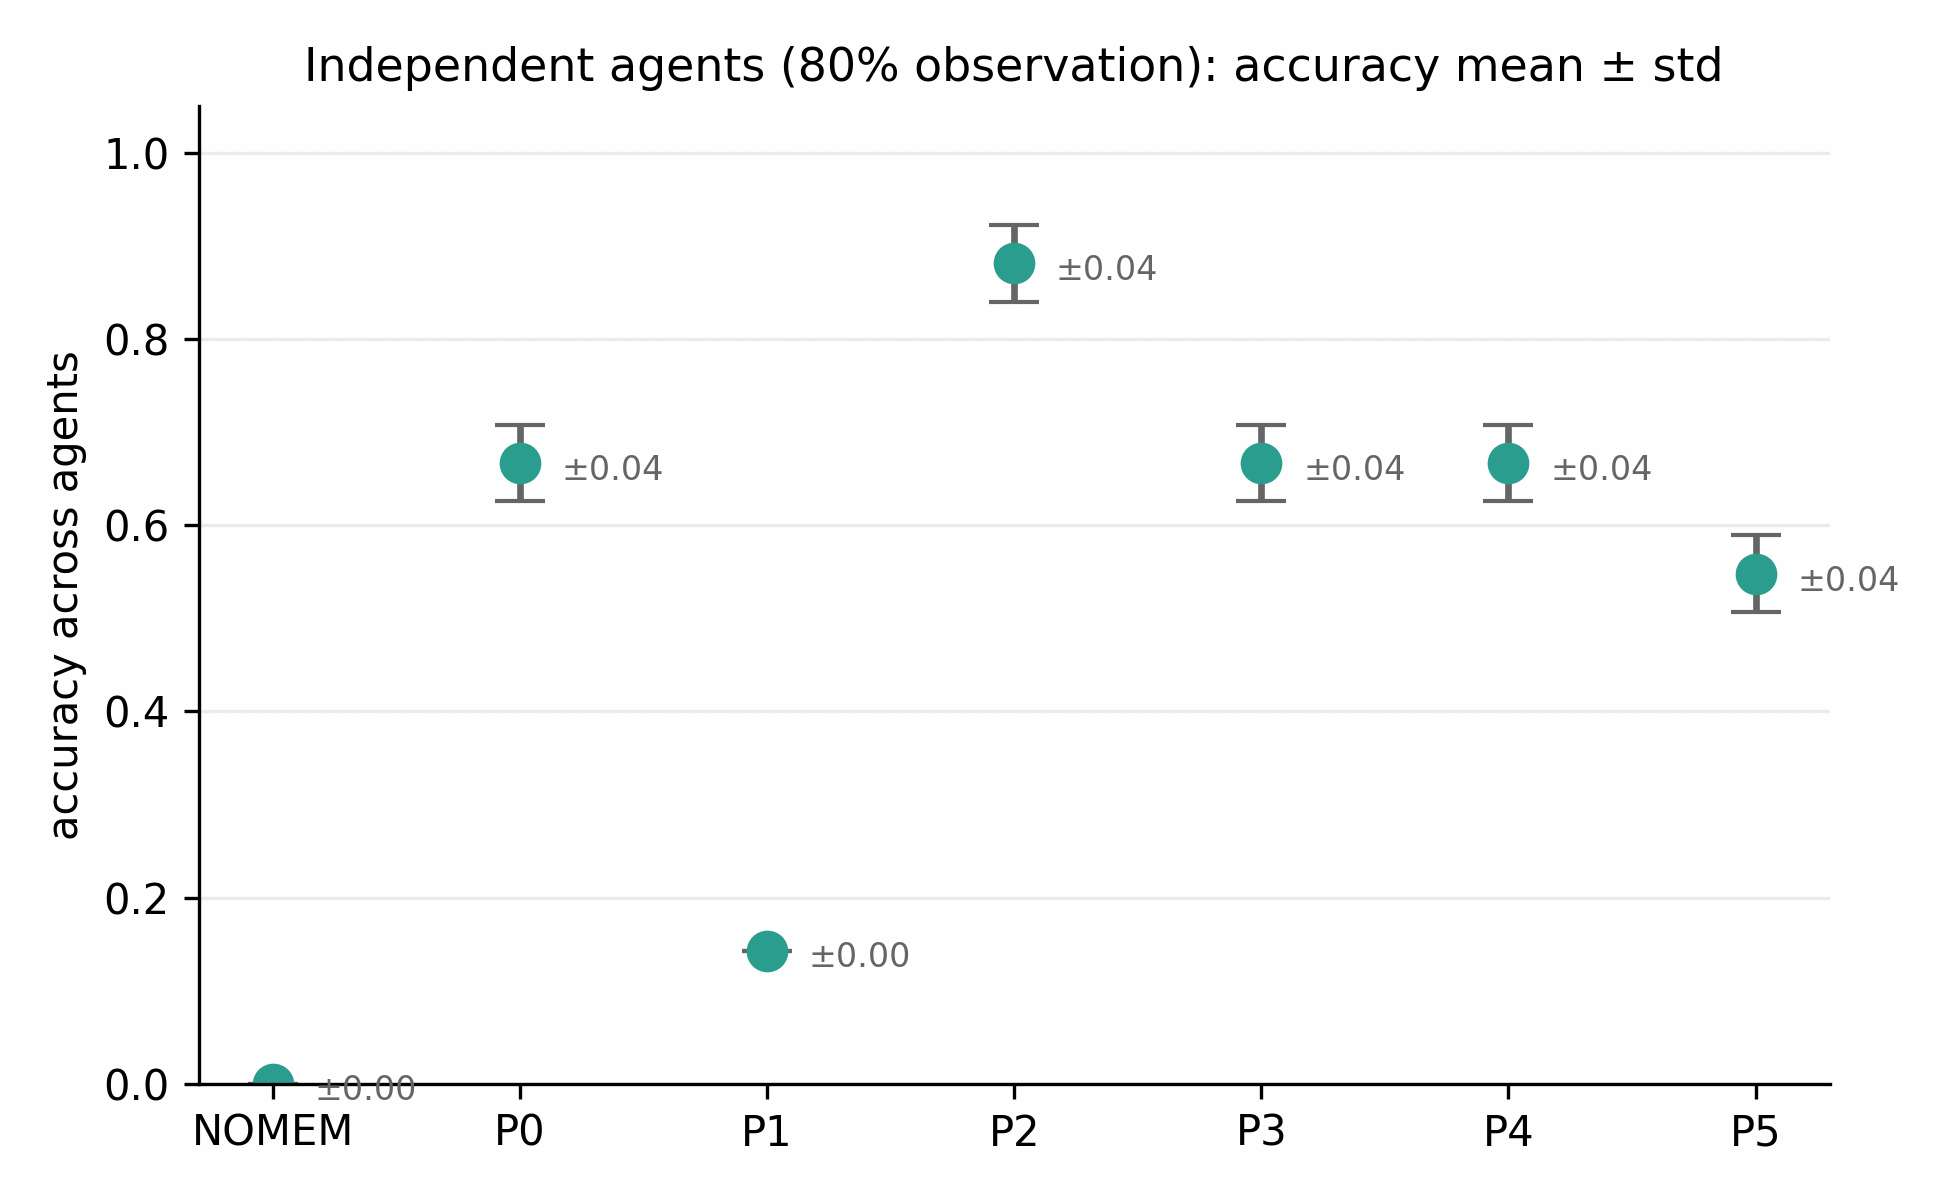
\includegraphics[width=0.7\textwidth]{figures/swarm_variance.png}
\caption{Mean and standard deviation of accuracy across the five independent agents in the independent topology.}
\label{fig:swarm-variance}
\end{figure}

\subsection{A Real-Data Pilot on the Shared Topology}
\label{sec:rq4-pilot}

A partial real-data campaign was run on the shared topology using MQuAKE-T and five heterogeneous extraction models, one per writer agent: GLM-5.2, MiniMax-M3, Gemini-3.1-Flash-Lite, Nemotron-3-Ultra, and Hunyuan, with GLM-5.2 as the shared answer model. Owing to the wall-clock cost of the P4 and P5 policies at this sample size, the pilot covers five of seven policies (NOMEM, P0, P1, P2, P3) on one of three topologies rather than the full matrix. Table~\ref{tab:rq4-pilot} reports the results.

\begin{table}[H]
\centering
\caption{Real-data pilot, shared topology, MQuAKE-T, 96 questions, five heterogeneous extraction models.}
\label{tab:rq4-pilot}
\small
\begin{tabular}{lccccc}
\toprule
Policy & Accuracy & Staleness & Tok/q & Invalidations & Active facts \\
\midrule
NOMEM & 0.000 & 0.000 & 156 & 0 & 140 \\
P0 & 0.333 & 0.271 & 710 & 0 & 140 \\
P1 (TTL 20d) & 0.281 & 0.135 & 729 & 0 & 79 \\
P2 & 0.365 & 0.271 & 710 & 0 & 140 \\
P3 & 0.365 & 0.271 & 710 & 0 & 140 \\
\bottomrule
\end{tabular}
\end{table}

The invalidation column is the finding. In the single-agent runs, one consistent extraction model per cell, P2 closes dozens of valid-time windows on MQuAKE-T (Section~\ref{sec:rq1}). Here, with five different models extracting from the same sessions, P2 records zero invalidations, and its retained-fact count, 140 active and 0 pruned, is identical to P0's. P2 and P3 track P0 to within 3.2 accuracy points, a gap the judge-reliability audit in Section~\ref{sec:judge-audit} already established as inside single-provider judge noise at this sample size, so the honest reading is that all three are statistically indistinguishable in this cell: bitemporal invalidation did not engage.

The mechanism is visible directly in the saved graph. Of 140 stored facts spanning 30 distinct predicate strings, the same underlying relation is extracted under multiple surface forms depending on which model wrote it: \texttt{head\_of\_government} (28 occurrences), \texttt{is\_head\_of\_government\_of} (9), and \texttt{head\_of\_government\_of} (7) all co-occur for what MQuAKE-T's schema treats as one functional predicate, and the same pattern appears on \texttt{citizen\_of} (32) versus \texttt{is\_citizen\_of} (6) versus \texttt{citizenship} (5). P2's contradiction detection matches on subject and predicate string; a correction extracted under a different surface form than the fact it corrects never triggers a match, so the valid-time window never closes. Only 3 of 137 subjects in the graph carry more than one fact at all, each exactly 2, versus the dozens of multi-fact subjects typical of the single-extractor single-agent runs, consistent with the same real-world relation being scattered across string variants rather than consolidated onto one.

P1 is the one policy in this pilot whose staleness reduction survives extraction heterogeneity, 0.135 versus P0's 0.271, because time-to-live pruning keys on \texttt{t\_valid\_start} alone and never needs two facts to agree on a predicate string to act. That protection is not free: P1 also prunes facts that were never superseded, and its accuracy, 0.281, is the lowest of the four non-floor policies in this pilot.

This pilot does not overturn the single-agent findings above; it identifies a boundary condition on them. P2's advantage over P0 was established, and holds, when one extractor is responsible for the graph's predicate vocabulary. It is not yet established for the heterogeneous-extractor case this pilot probes, and the mechanism above, predicate-string fragmentation defeating exact-match contradiction detection, is a directly observed explanation rather than a speculative one. A canonicalization step ahead of the write-time match, mapping extracted predicate strings to a fixed schema or matching on embedding similarity rather than string equality, is the natural fix and is noted as future work in Chapter~\ref{chap:discussion}. The remaining sixteen cells of the full twenty-one-cell matrix, both remaining topologies plus P4 and P5 on the shared topology, were not completed in the time available for this thesis; Table~\ref{tab:swarm-results} above remains the only evidence on the full seven-policy, three-topology design, and it is offline-synthetic.

\section{Memory Growth}
\label{sec:memory-growth}

Table~\ref{tab:memory-growth} reports the count of active facts in memory at five checkpoints across the 38 sessions of each benchmark, using the GLM-5.2 answer model.

\begin{table}[H]
\centering
\caption{Active fact count at session checkpoints.}
\label{tab:memory-growth}
\begin{tabular}{lccccc}
\toprule
& \multicolumn{5}{c}{FactConsolidation} \\
Policy & s1 & s10 & s20 & s30 & s38 \\
\midrule
P0 & 10 & 100 & 200 & 300 & 380 \\
P1 & 10 & 100 & 200 & 210 & 210 \\
P2 & 10 & 100 & 189 & 270 & 324 \\
P3 & 10 & 98 & 185 & 273 & 334 \\
P4 & 10 & 96 & 195 & 294 & 374 \\
P5 & 10 & 100 & 198 & 291 & 365 \\
\midrule
& \multicolumn{5}{c}{MQuAKE-T} \\
Policy & s1 & s10 & s20 & s30 & s38 \\
\midrule
P0 & 1 & 74 & 169 & 276 & 382 \\
P1 & 1 & 74 & 169 & 209 & 251 \\
P2 & 1 & 74 & 165 & 266 & 357 \\
P3 & 1 & 74 & 164 & 264 & 351 \\
P4 & 1 & 74 & 166 & 266 & 369 \\
P5 & 1 & 74 & 168 & 271 & 365 \\
\bottomrule
\end{tabular}
\end{table}

Two observations follow from this table. P1's curve flattens abruptly once its time-to-live horizon is reached, which is the direct cause of its accuracy collapse reported in Section~\ref{sec:headline}: it is discarding answerable facts wholesale once they cross the age threshold, rather than selectively discarding only facts that have actually been superseded. P2's curve, by contrast, tracks P0's closely for most of the run and diverges only gradually, which is exactly the shape one would expect from a policy that removes only what has genuinely become invalid rather than removing by a blunt criterion such as age.

\begin{figure}[H]
\centering
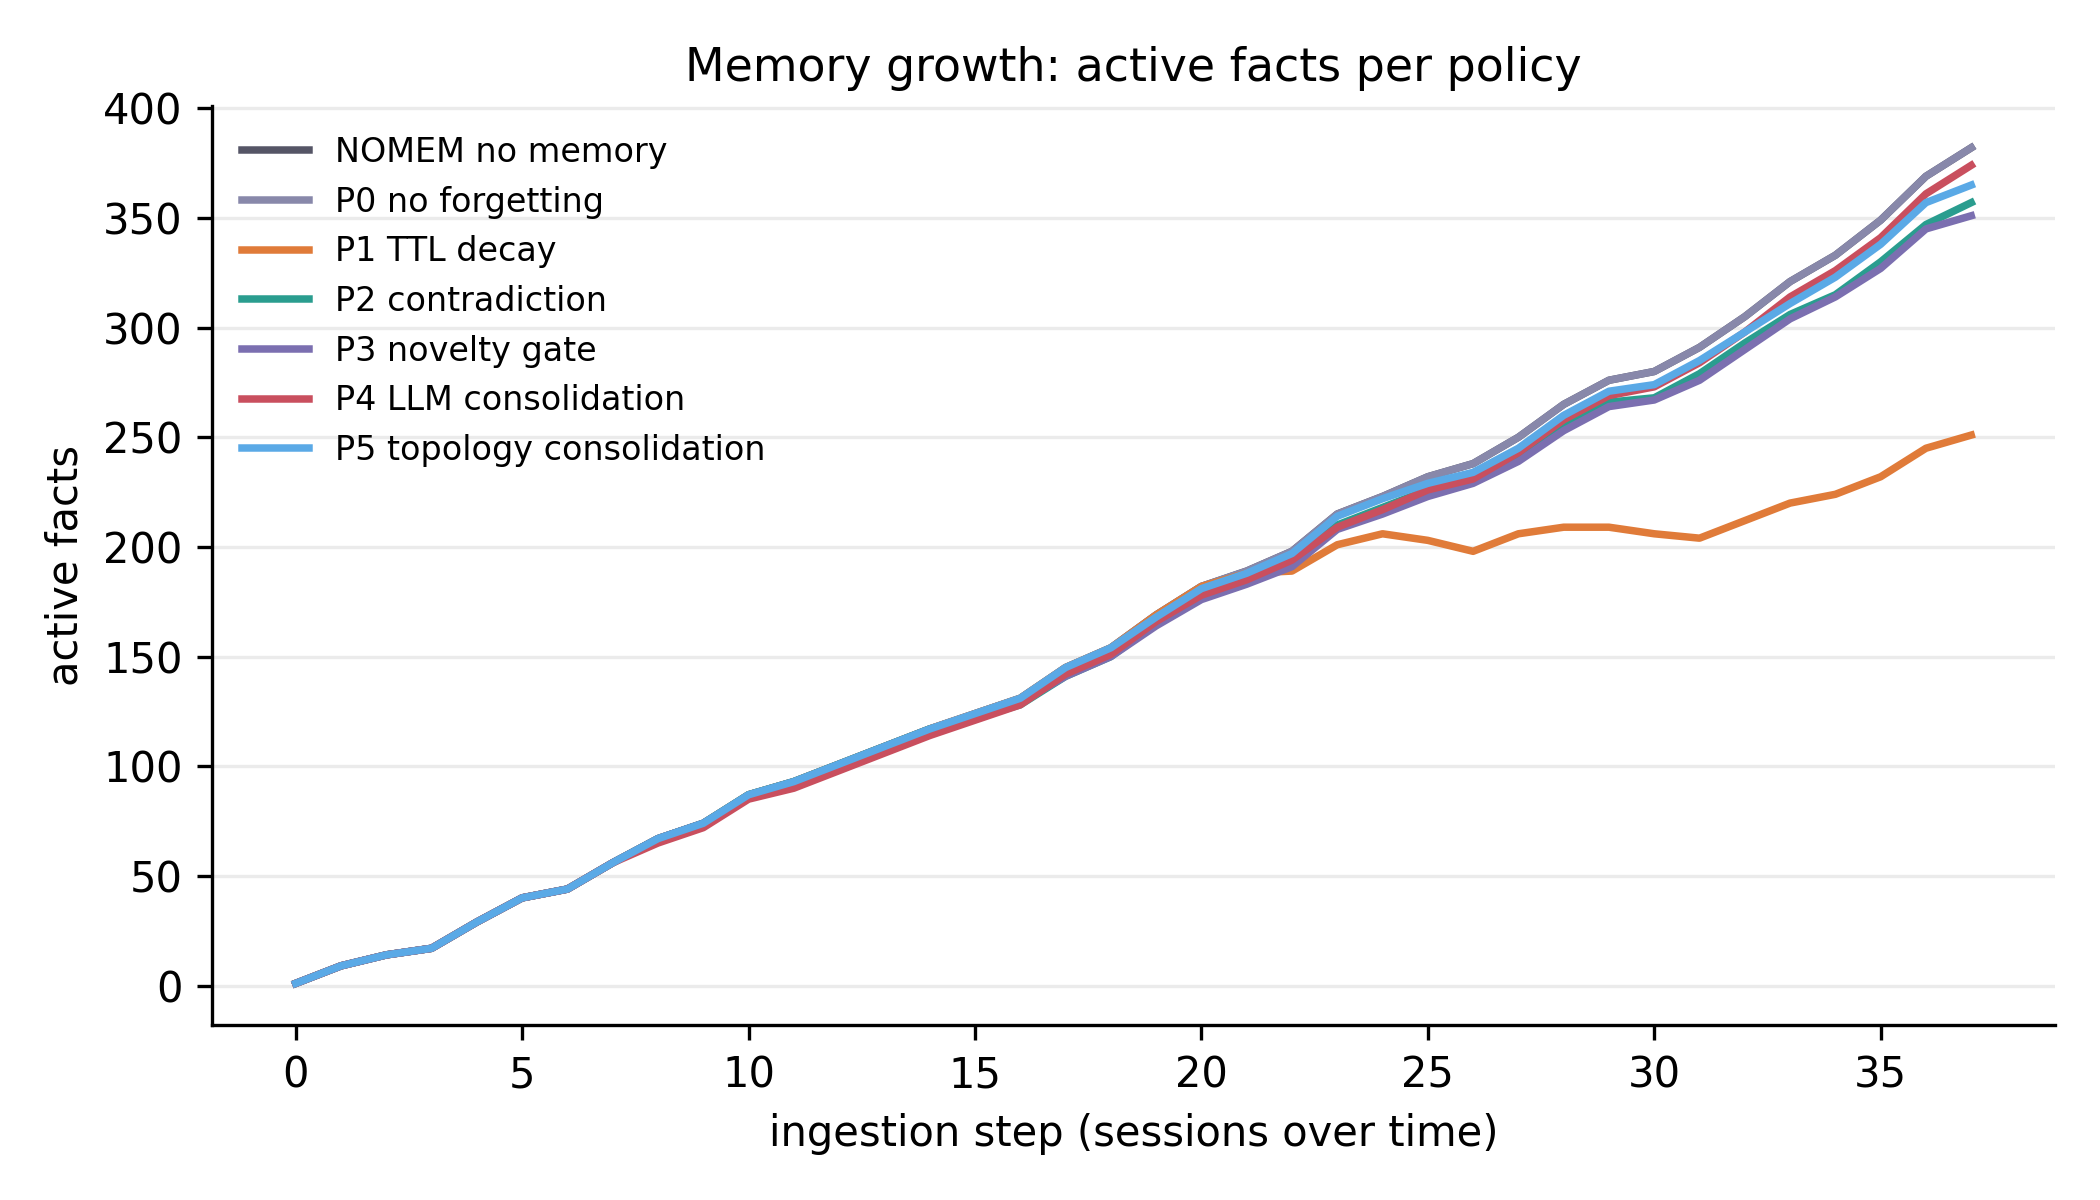
\includegraphics[width=0.75\textwidth]{figures/memory_growth_mquake_t.png}
\caption{Active fact count over the course of the 38 MQuAKE-T sessions, by policy.}
\label{fig:memory-growth}
\end{figure}

\section{Per-Model Breakdown}
\label{sec:per-model}

Table~\ref{tab:per-model} reports accuracy broken out by the two answer models used in this thesis, GLM-5.2 and MiniMax-M3, to check whether the policy effects reported above are an idiosyncrasy of a single answer model.

\begin{table}[H]
\centering
\caption{Accuracy by policy, broken out by answer model.}
\label{tab:per-model}
\begin{tabular}{lcccc}
\toprule
Policy & FC GLM-5.2 & FC MiniMax-M3 & MQ GLM-5.2 & MQ MiniMax-M3 \\
\midrule
NOMEM & 0.000 & 0.000 & 0.000 & 0.000 \\
P0 & 0.860 & 0.820 & 0.969 & 0.969 \\
P1 & 0.650 & 0.610 & 0.865 & 0.875 \\
P2 & 0.850 & 0.830 & 0.969 & 0.969 \\
P3 & 0.680 & 0.650 & 0.802 & 0.781 \\
P4 & 0.820 & 0.780 & 0.958 & 0.948 \\
P5 & 0.820 & 0.770 & 0.823 & 0.781 \\
\bottomrule
\end{tabular}
\end{table}

\begin{figure}[H]
\centering
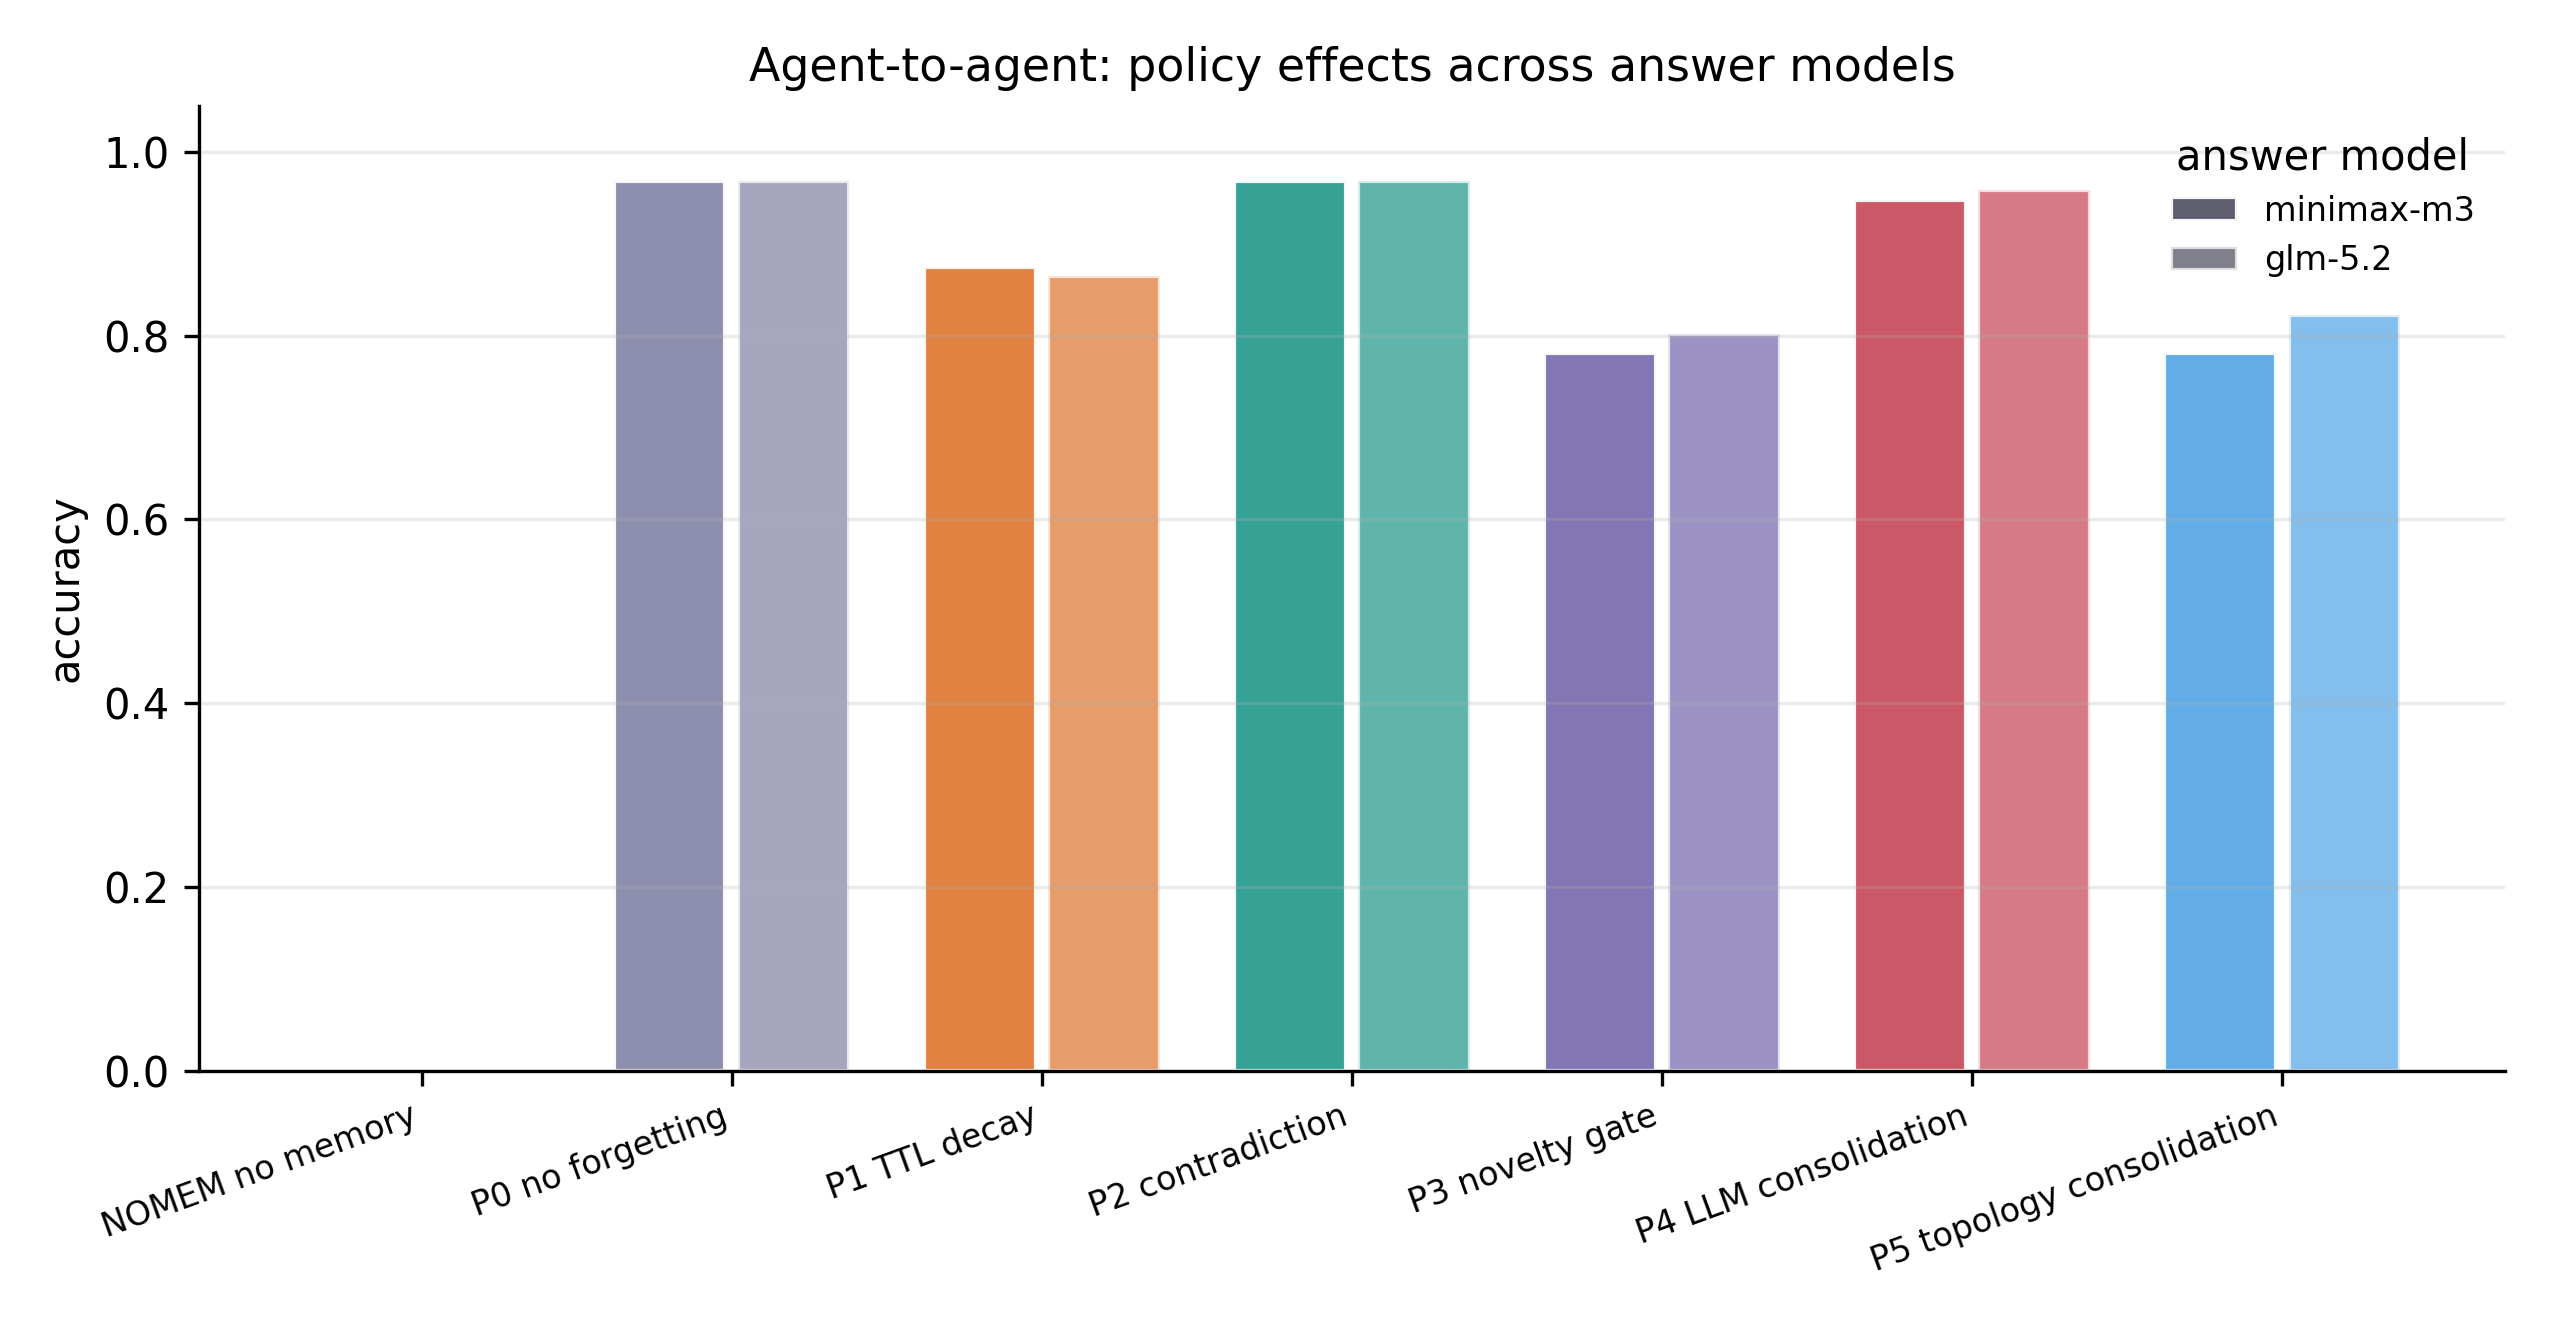
\includegraphics[width=0.75\textwidth]{figures/model_comparison_mquake_t.png}
\caption{Accuracy by policy, broken out by answer model, MQuAKE-T.}
\label{fig:model-comparison}
\end{figure}

Both answer models rank all seven policies in the identical order. Token-F1, not shown in this table, diverges sharply between the two models, for example 0.973 against 0.622 for P0 on MQuAKE-T, because MiniMax-M3 tends to answer more verbosely and token-F1 penalizes length directly. Accuracy, which is scored semantically by a judge rather than by lexical overlap, agrees closely between the two models despite this divergence in verbosity. This is itself a small methodological observation worth stating explicitly: token-F1 should not be relied upon as a primary metric when comparing models with substantially different verbosity profiles, precisely because it can disagree with a semantic judgment for reasons unrelated to correctness.
